\chapter{Density Plots}\label{density-plots}

In this part, we will work towards creating the density plot below. We
will take you from a basic density plot and explain all the
customisations we add to the code step-by-step.

\begin{center}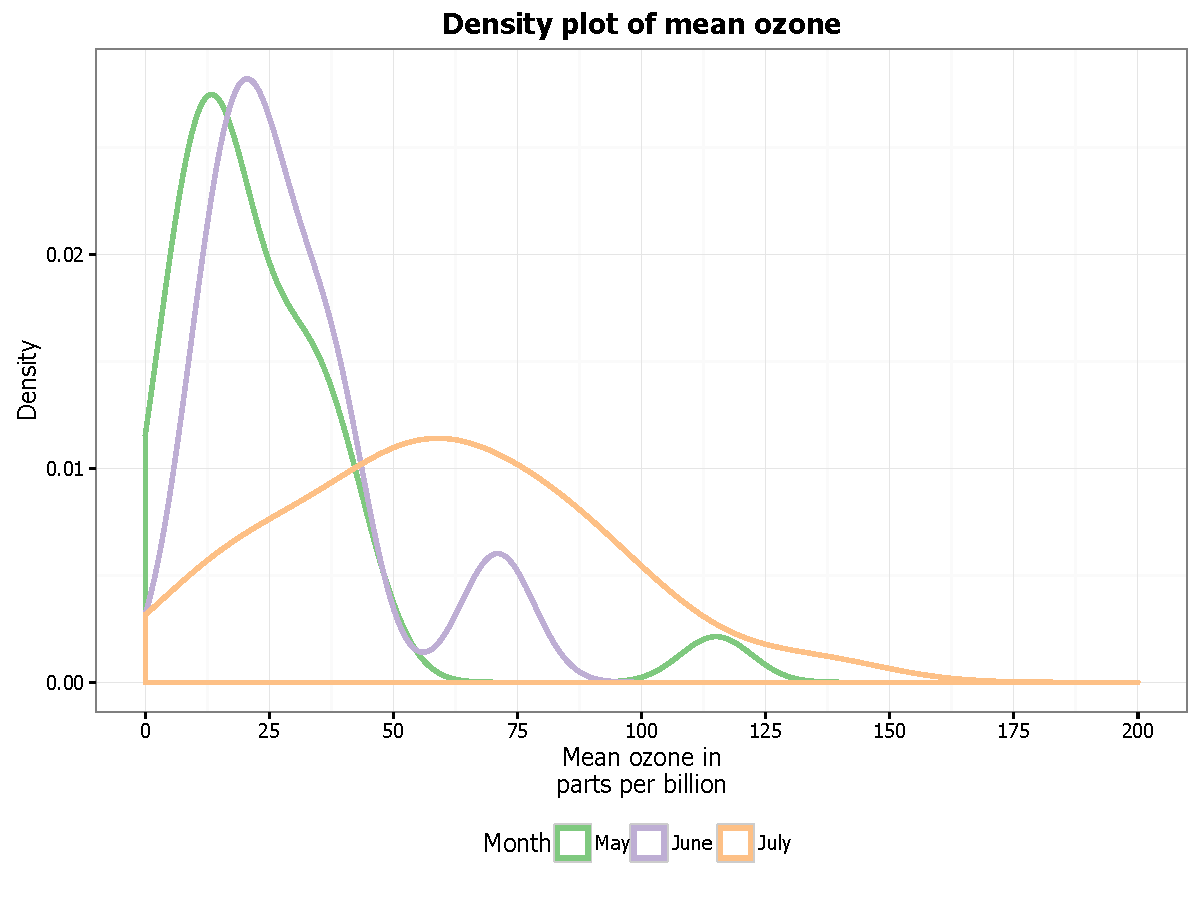
\includegraphics[width=0.55\linewidth]{figures/density_final-1} \end{center}

The first thing to do is load in the data, as below:

\begin{Shaded}
\begin{Highlighting}[]
\KeywordTok{rm}\NormalTok{(}\DataTypeTok{list =} \KeywordTok{ls}\NormalTok{())}
\KeywordTok{library}\NormalTok{(datasets)}
\KeywordTok{library}\NormalTok{(ggplot2)}

\KeywordTok{data}\NormalTok{(airquality)}
\end{Highlighting}
\end{Shaded}

\section{Basic density plot}\label{basic-density-plot}

In order to initialise a plot we tell ggplot that \texttt{airquality} is
our data, and specify that our x axis plots the \texttt{Ozone} variable.
We then instruct ggplot to render this as a density plot by adding the
\texttt{geom\_density()} option.

\begin{Shaded}
\begin{Highlighting}[]
\NormalTok{p8 <-}\StringTok{ }\KeywordTok{ggplot}\NormalTok{(airquality, }\KeywordTok{aes}\NormalTok{(}\DataTypeTok{x =} \NormalTok{Ozone)) +}\StringTok{ }\KeywordTok{geom_density}\NormalTok{()}
\NormalTok{p8}
\end{Highlighting}
\end{Shaded}

\begin{center}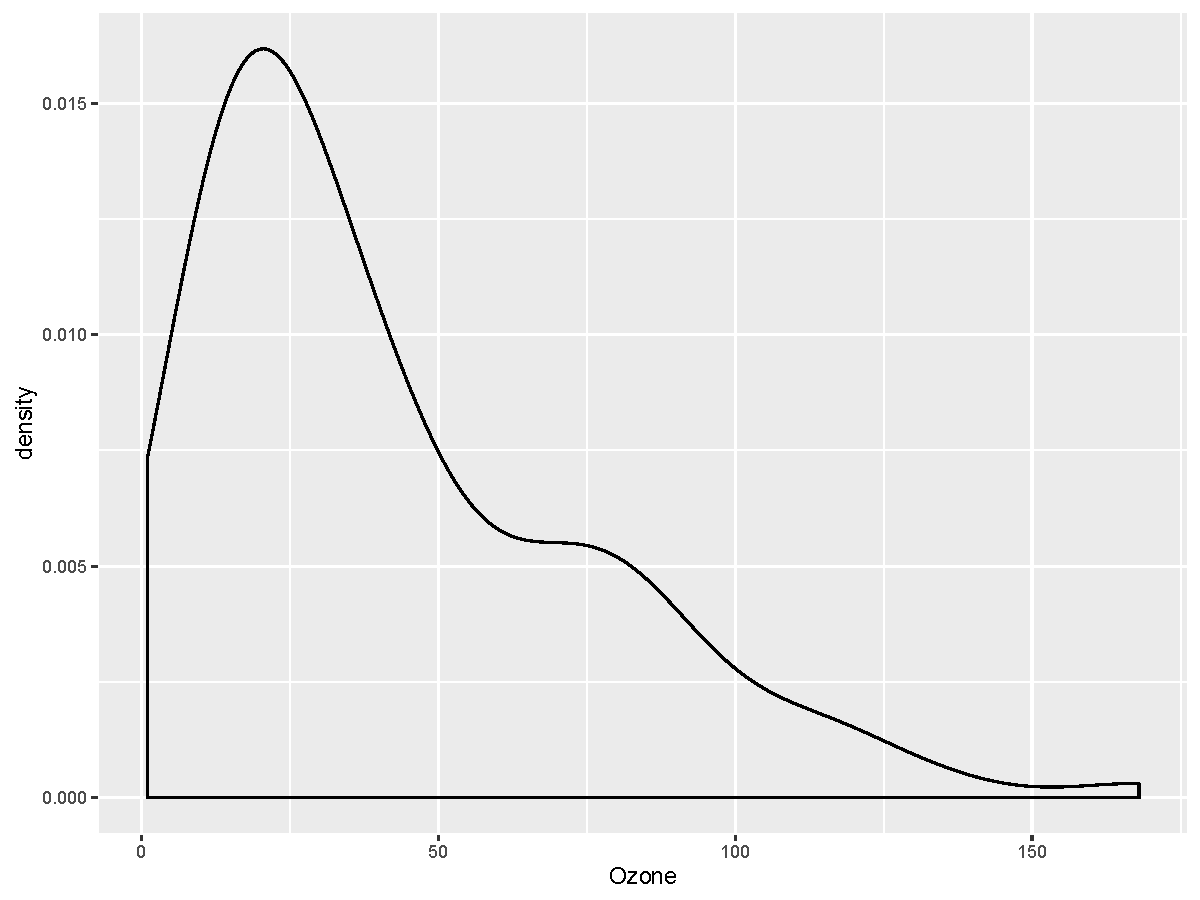
\includegraphics[width=0.55\linewidth]{figures/density_1-1} \end{center}

\section{Customising axis labels}\label{customising-axis-labels-1}

In order to change the axis labels, we have a couple of options. In this
case, we have used the \texttt{scale\_x\_continuous} and
\texttt{scale\_y\_continuous} options, as these have further
customisation options for the axes we will use below. In each, we add
the desired name to the \texttt{name} argument as a string.

\begin{Shaded}
\begin{Highlighting}[]
\NormalTok{p8 <-}\StringTok{ }\NormalTok{p8 +}\StringTok{ }\KeywordTok{scale_x_continuous}\NormalTok{(}\DataTypeTok{name =} \StringTok{"Mean ozone in parts per billion"}\NormalTok{) +}
\StringTok{      }\KeywordTok{scale_y_continuous}\NormalTok{(}\DataTypeTok{name =} \StringTok{"Density"}\NormalTok{)}
\NormalTok{p8}
\end{Highlighting}
\end{Shaded}

\begin{center}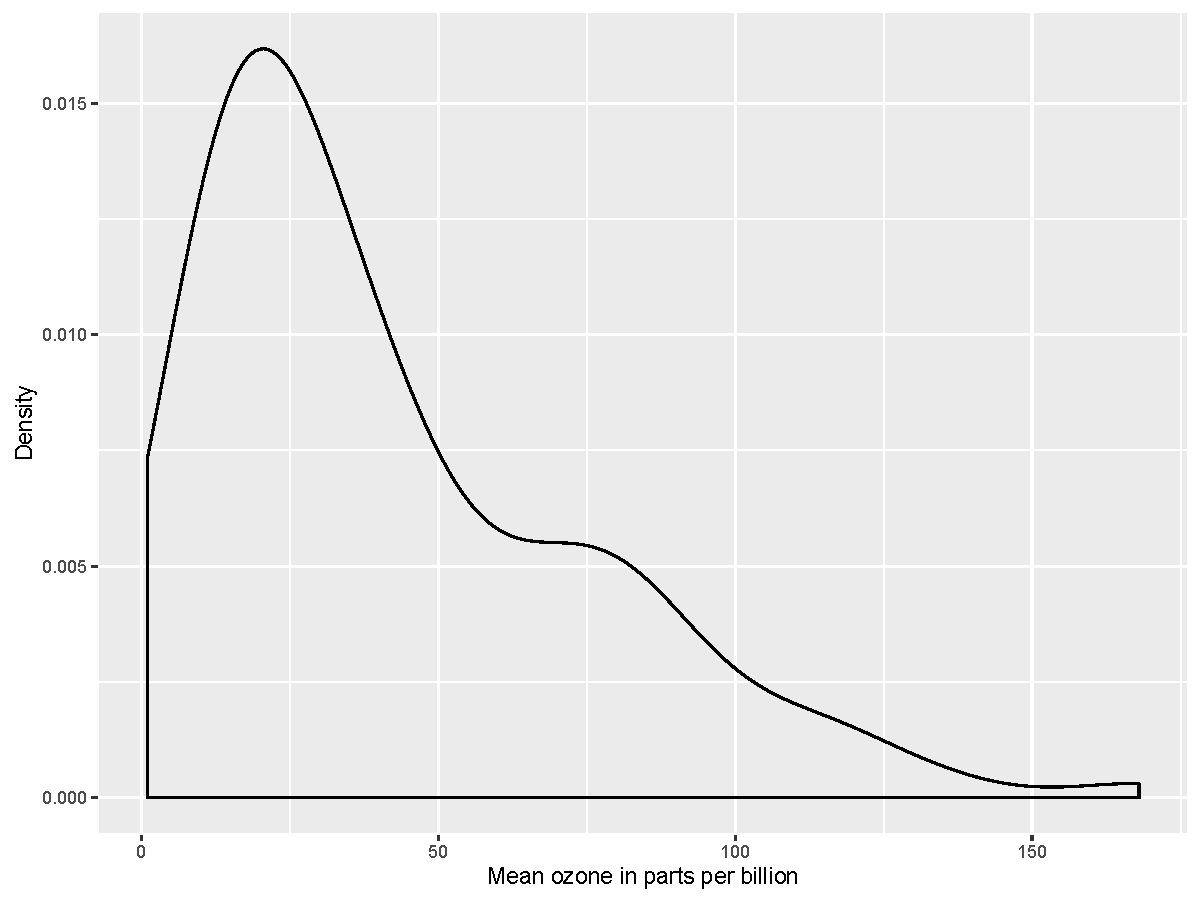
\includegraphics[width=0.55\linewidth]{figures/density_2-1} \end{center}

ggplot also allows for the use of multiline names (in both axes and
titles). Here, we've changed the x-axis label so that it goes over two
lines using the \texttt{\textbackslash{}n} character to break the line.

\begin{Shaded}
\begin{Highlighting}[]
\NormalTok{p8 <-}\StringTok{ }\NormalTok{p8 +}\StringTok{ }\KeywordTok{scale_x_continuous}\NormalTok{(}\DataTypeTok{name =} \StringTok{"Mean ozone in}\CharTok{\textbackslash{}n}\StringTok{parts per billion"}\NormalTok{)}
\NormalTok{p8}
\end{Highlighting}
\end{Shaded}

\begin{center}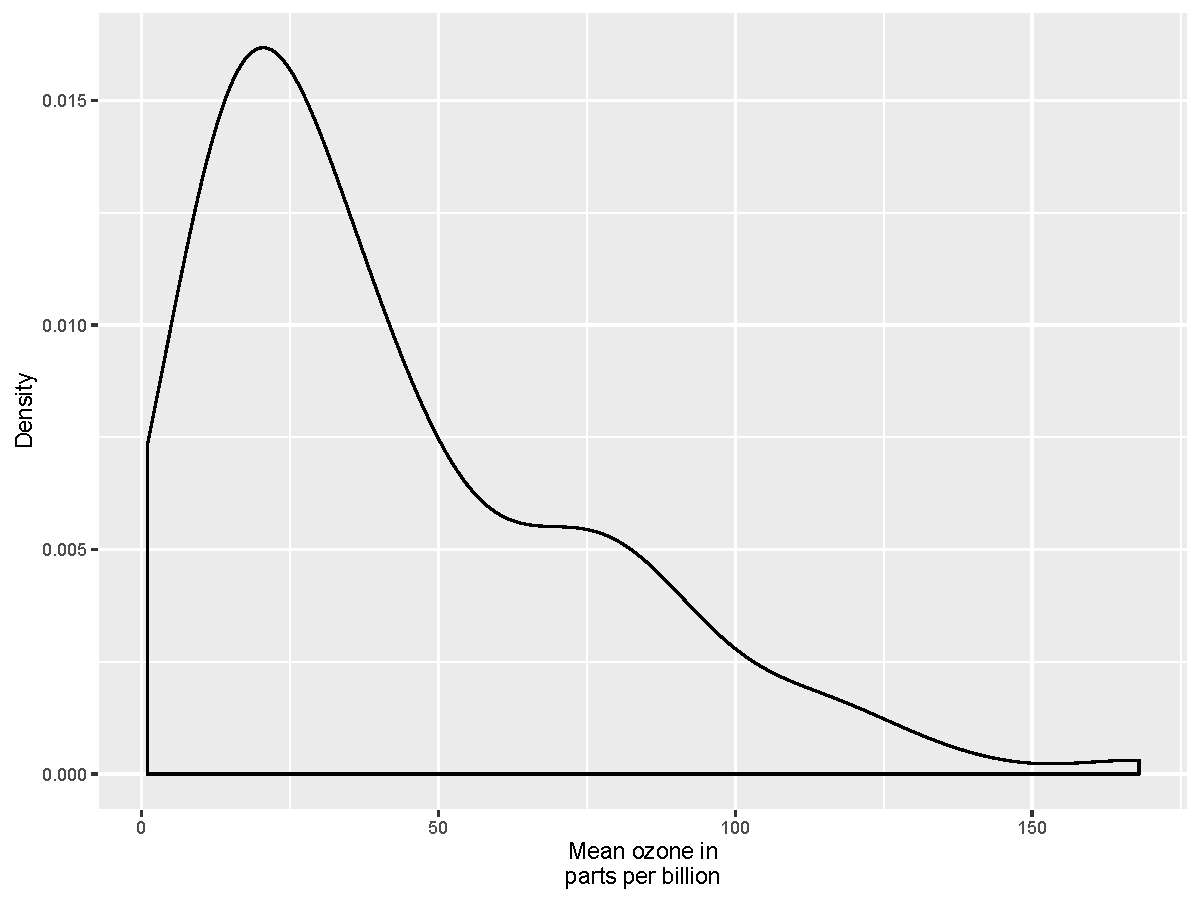
\includegraphics[width=0.55\linewidth]{figures/density_3-1} \end{center}

\section{Changing axis ticks}\label{changing-axis-ticks-1}

The next thing we will change is the axis ticks. Let's make the x-axis
ticks appear at every 25 units rather than 50 using the
\texttt{breaks\ =\ seq(0,\ 200,\ 25)} argument in
\texttt{scale\_x\_continuous}. (The \texttt{seq} function is a base R
function that indicates the start and endpoints and the units to
increment by respectively. See \texttt{help(seq)} for more information.)
We ensure that the x-axis begins and ends where we want by also adding
the argument \texttt{limits\ =\ c(0,\ 200)} to
\texttt{scale\_x\_continuous}.

\begin{Shaded}
\begin{Highlighting}[]
\NormalTok{p8 <-}\StringTok{ }\NormalTok{p8 +}\StringTok{ }\KeywordTok{scale_x_continuous}\NormalTok{(}\DataTypeTok{name =} \StringTok{"Mean ozone in}\CharTok{\textbackslash{}n}\StringTok{parts per billion"}\NormalTok{,}
\StringTok{        }\DataTypeTok{breaks =} \KeywordTok{seq}\NormalTok{(}\DecValTok{0}\NormalTok{, }\DecValTok{200}\NormalTok{, }\DecValTok{25}\NormalTok{),}
\StringTok{        }\DataTypeTok{limits=}\KeywordTok{c}\NormalTok{(}\DecValTok{0}\NormalTok{, }\DecValTok{200}\NormalTok{))}
\NormalTok{p8}
\end{Highlighting}
\end{Shaded}

\begin{center}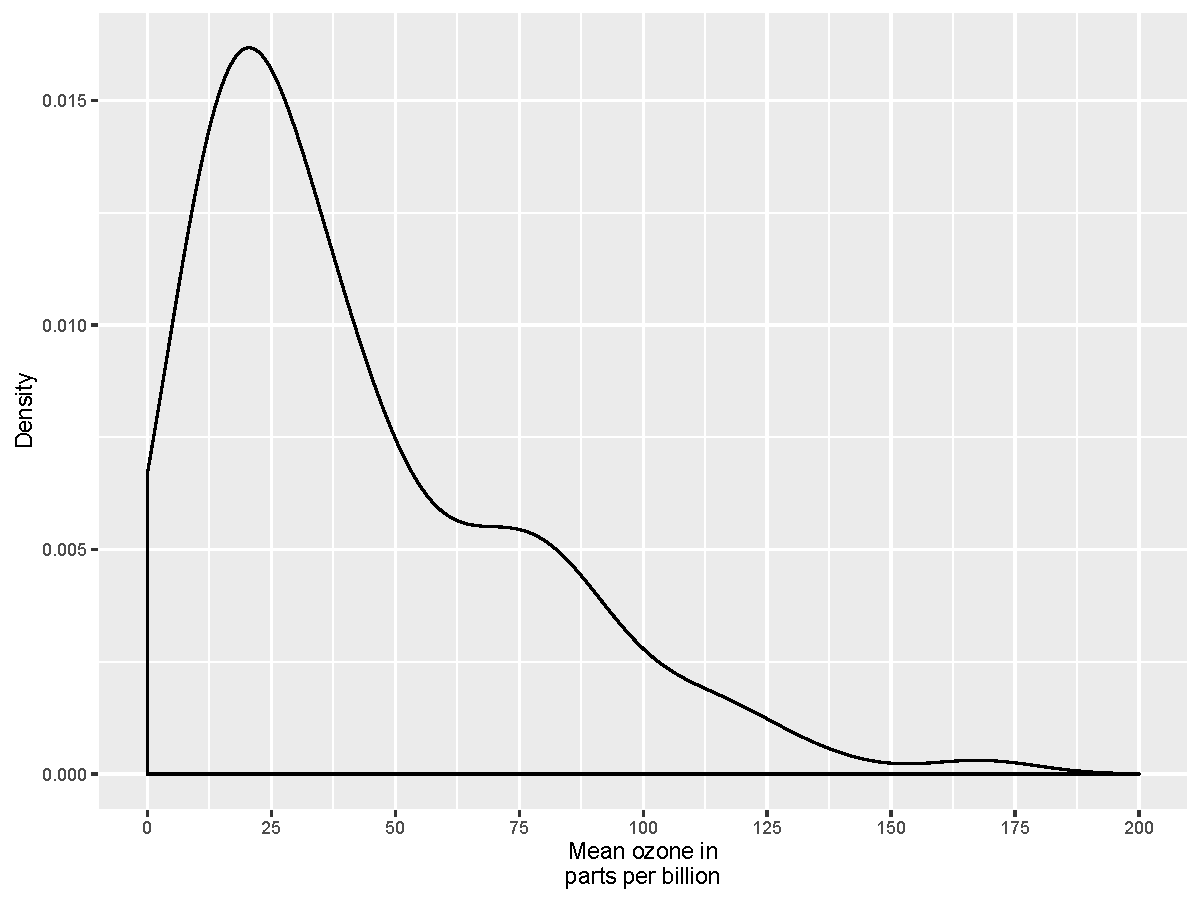
\includegraphics[width=0.55\linewidth]{figures/density_4-1} \end{center}

\section{Adding a title}\label{adding-a-title-1}

To add a title, we include the option \texttt{ggtitle} and include the
name of the graph as a string argument.

\begin{Shaded}
\begin{Highlighting}[]
\NormalTok{p8 <-}\StringTok{ }\NormalTok{p8 +}\StringTok{ }\KeywordTok{ggtitle}\NormalTok{(}\StringTok{"Density plot of mean ozone"}\NormalTok{)}
\NormalTok{p8}
\end{Highlighting}
\end{Shaded}

\begin{center}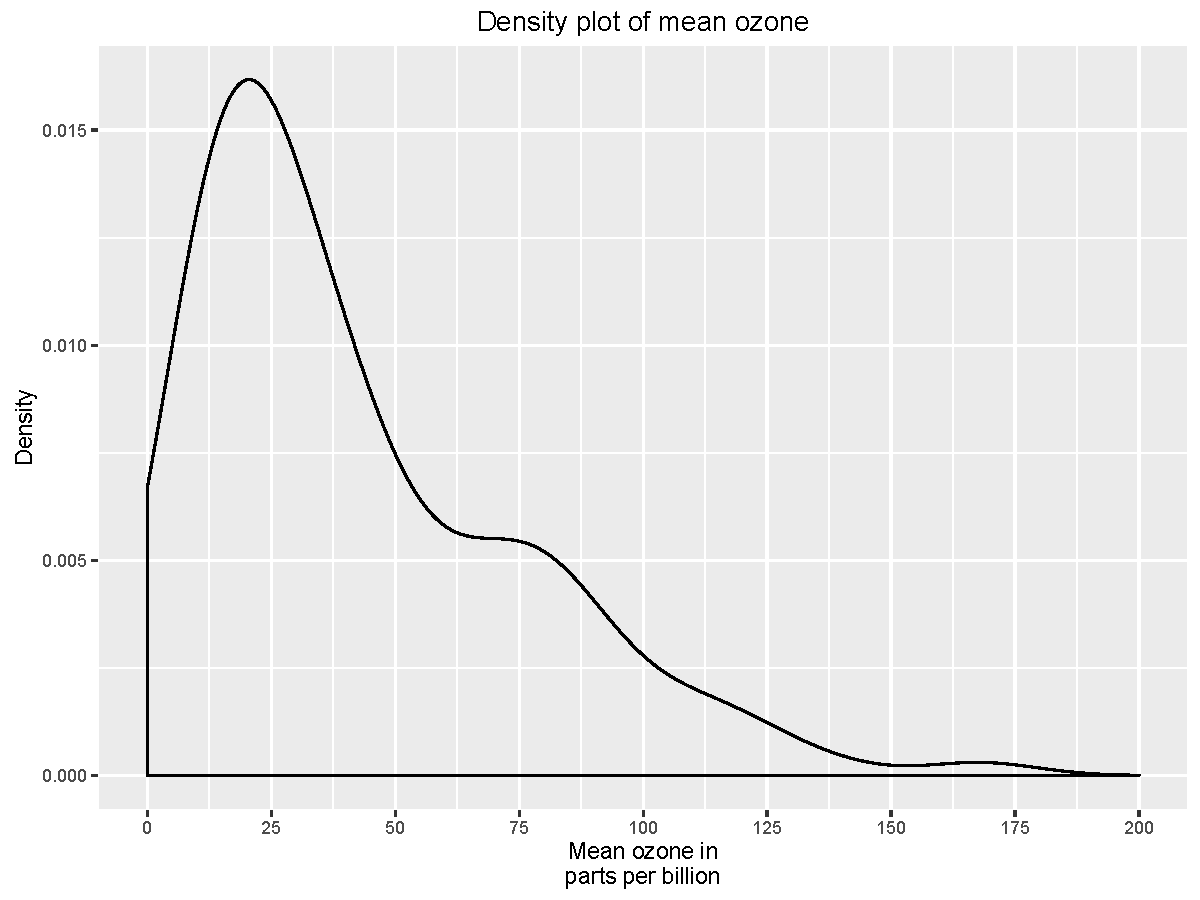
\includegraphics[width=0.55\linewidth]{figures/density_5-1} \end{center}

\section{Changing the colour of the
curves}\label{changing-the-colour-of-the-curves}

To change the line and fill colours of the density plot, we add a valid
colour to the \texttt{colour} and \texttt{fill} arguments in
\texttt{geom\_density()} (note that I assigned these colours to
variables outside of the plot to make it easier to change them). A list
of valid colours is
\href{http://www.stat.columbia.edu/~tzheng/files/Rcolor.pdf}{here}.

\begin{Shaded}
\begin{Highlighting}[]
\NormalTok{fill <-}\StringTok{ "gold1"}
\NormalTok{line <-}\StringTok{ "goldenrod2"}

\NormalTok{p8 <-}\StringTok{ }\KeywordTok{ggplot}\NormalTok{(airquality, }\KeywordTok{aes}\NormalTok{(}\DataTypeTok{x =} \NormalTok{Ozone)) +}\StringTok{ }
\StringTok{      }\KeywordTok{geom_density}\NormalTok{(}\DataTypeTok{fill =} \NormalTok{fill, }\DataTypeTok{colour =} \NormalTok{line) +}
\StringTok{      }\KeywordTok{scale_x_continuous}\NormalTok{(}\DataTypeTok{name =} \StringTok{"Mean ozone in}\CharTok{\textbackslash{}n}\StringTok{parts per billion"}\NormalTok{,}
\StringTok{        }\DataTypeTok{breaks =} \KeywordTok{seq}\NormalTok{(}\DecValTok{0}\NormalTok{, }\DecValTok{200}\NormalTok{, }\DecValTok{25}\NormalTok{),}
\StringTok{        }\DataTypeTok{limits=}\KeywordTok{c}\NormalTok{(}\DecValTok{0}\NormalTok{, }\DecValTok{200}\NormalTok{)) +}
\StringTok{      }\KeywordTok{scale_y_continuous}\NormalTok{(}\DataTypeTok{name =} \StringTok{"Density"}\NormalTok{) +}
\StringTok{      }\KeywordTok{ggtitle}\NormalTok{(}\StringTok{"Density plot of mean ozone"}\NormalTok{)}
\NormalTok{p8}
\end{Highlighting}
\end{Shaded}

\begin{center}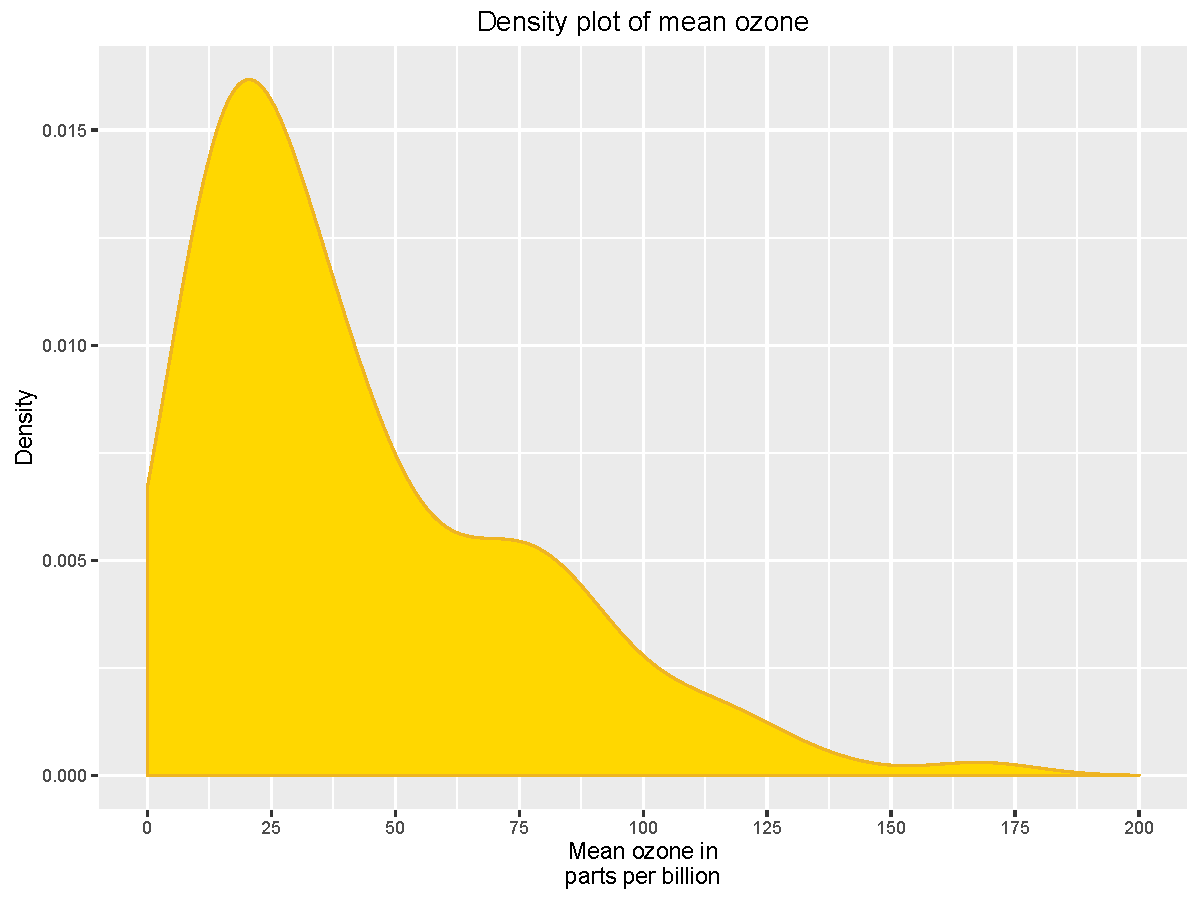
\includegraphics[width=0.55\linewidth]{figures/density_6-1} \end{center}

If you want to go beyond the options in the list above, you can also
specify exact HEX colours by including them as a string preceded by a
hash, e.g., ``\#FFFFFF''. Below, we have called two shades of blue for
the fill and lines using their HEX codes.

\begin{Shaded}
\begin{Highlighting}[]
\NormalTok{fill <-}\StringTok{ "#4271AE"}
\NormalTok{line <-}\StringTok{ "#1F3552"}

\NormalTok{p8 <-}\StringTok{ }\KeywordTok{ggplot}\NormalTok{(airquality, }\KeywordTok{aes}\NormalTok{(}\DataTypeTok{x =} \NormalTok{Ozone)) +}\StringTok{ }
\StringTok{      }\KeywordTok{geom_density}\NormalTok{(}\DataTypeTok{fill =} \NormalTok{fill, }\DataTypeTok{colour =} \NormalTok{line) +}
\StringTok{      }\KeywordTok{scale_x_continuous}\NormalTok{(}\DataTypeTok{name =} \StringTok{"Mean ozone in}\CharTok{\textbackslash{}n}\StringTok{parts per billion"}\NormalTok{,}
\StringTok{        }\DataTypeTok{breaks =} \KeywordTok{seq}\NormalTok{(}\DecValTok{0}\NormalTok{, }\DecValTok{200}\NormalTok{, }\DecValTok{25}\NormalTok{),}
\StringTok{        }\DataTypeTok{limits=}\KeywordTok{c}\NormalTok{(}\DecValTok{0}\NormalTok{, }\DecValTok{200}\NormalTok{)) +}
\StringTok{      }\KeywordTok{scale_y_continuous}\NormalTok{(}\DataTypeTok{name =} \StringTok{"Density"}\NormalTok{) +}
\StringTok{      }\KeywordTok{ggtitle}\NormalTok{(}\StringTok{"Density plot of mean ozone"}\NormalTok{)}
\NormalTok{p8}
\end{Highlighting}
\end{Shaded}

\begin{center}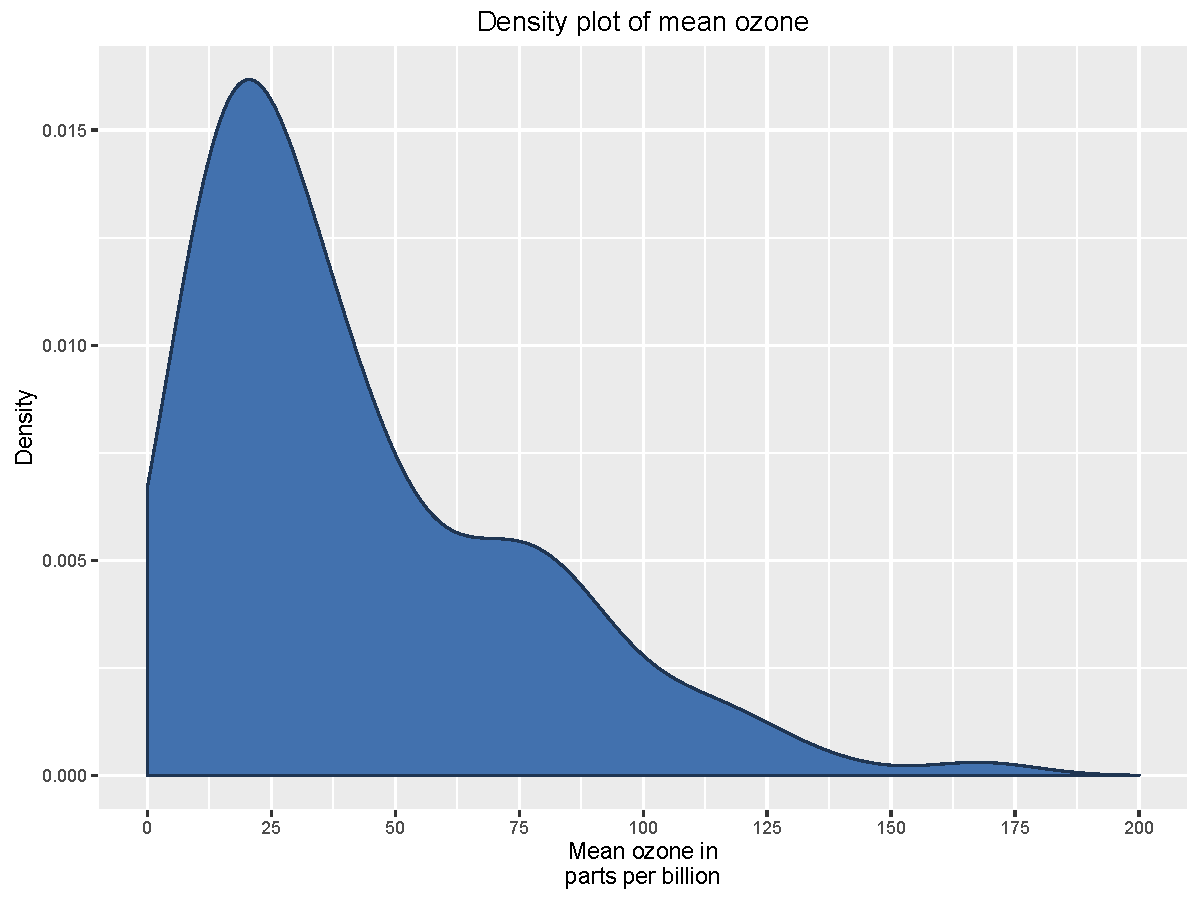
\includegraphics[width=0.55\linewidth]{figures/density_7-1} \end{center}

You can also specify the degree of transparency in the density fill area
using the argument \texttt{alpha} in \texttt{geom\_density}. This ranges
from 0 to 1.

\begin{Shaded}
\begin{Highlighting}[]
\NormalTok{p8 <-}\StringTok{ }\KeywordTok{ggplot}\NormalTok{(airquality, }\KeywordTok{aes}\NormalTok{(}\DataTypeTok{x =} \NormalTok{Ozone)) +}\StringTok{ }
\StringTok{      }\KeywordTok{geom_density}\NormalTok{(}\DataTypeTok{fill =} \NormalTok{fill, }\DataTypeTok{colour =} \NormalTok{line,}
\StringTok{        }\DataTypeTok{alpha =} \FloatTok{0.6}\NormalTok{) +}
\StringTok{      }\KeywordTok{scale_x_continuous}\NormalTok{(}\DataTypeTok{name =} \StringTok{"Mean ozone in}\CharTok{\textbackslash{}n}\StringTok{parts per billion"}\NormalTok{,}
\StringTok{        }\DataTypeTok{breaks =} \KeywordTok{seq}\NormalTok{(}\DecValTok{0}\NormalTok{, }\DecValTok{200}\NormalTok{, }\DecValTok{25}\NormalTok{),}
\StringTok{        }\DataTypeTok{limits=}\KeywordTok{c}\NormalTok{(}\DecValTok{0}\NormalTok{, }\DecValTok{200}\NormalTok{)) +}
\StringTok{      }\KeywordTok{scale_y_continuous}\NormalTok{(}\DataTypeTok{name =} \StringTok{"Density"}\NormalTok{) +}
\StringTok{      }\KeywordTok{ggtitle}\NormalTok{(}\StringTok{"Density plot of mean ozone"}\NormalTok{)}
\NormalTok{p8}
\end{Highlighting}
\end{Shaded}

\begin{center}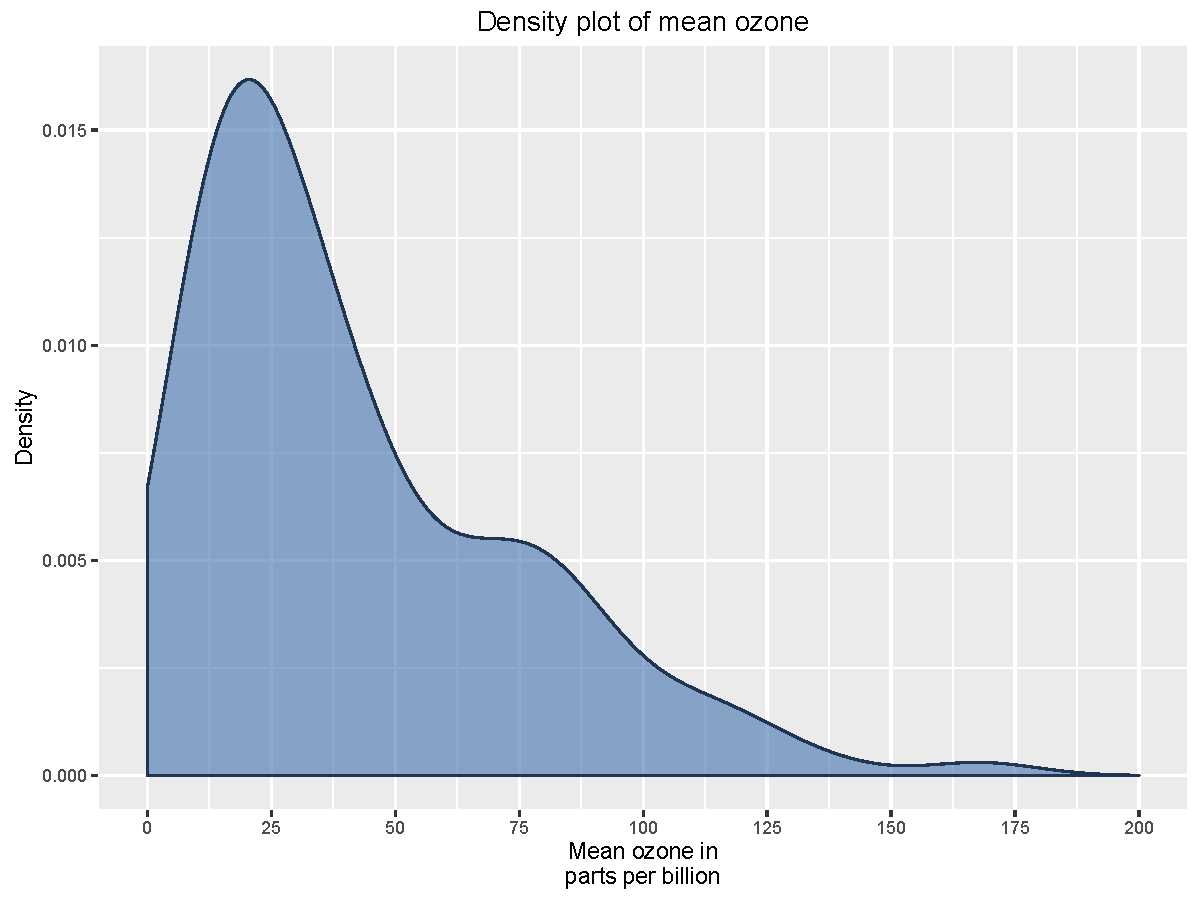
\includegraphics[width=0.55\linewidth]{figures/density_8-1} \end{center}

\section{Using the white theme}\label{using-the-white-theme-7}

As explained in the previous posts, we can also change the overall look
of the plot using themes. We'll start using a simple theme customisation
by adding \texttt{theme\_bw()}. As you can see, we can further tweak the
graph using the \texttt{theme} option, which we've used so far to change
the legend.

\begin{Shaded}
\begin{Highlighting}[]
\NormalTok{p8 <-}\StringTok{ }\NormalTok{p8 +}\StringTok{ }\KeywordTok{theme_bw}\NormalTok{()}
\NormalTok{p8}
\end{Highlighting}
\end{Shaded}

\begin{center}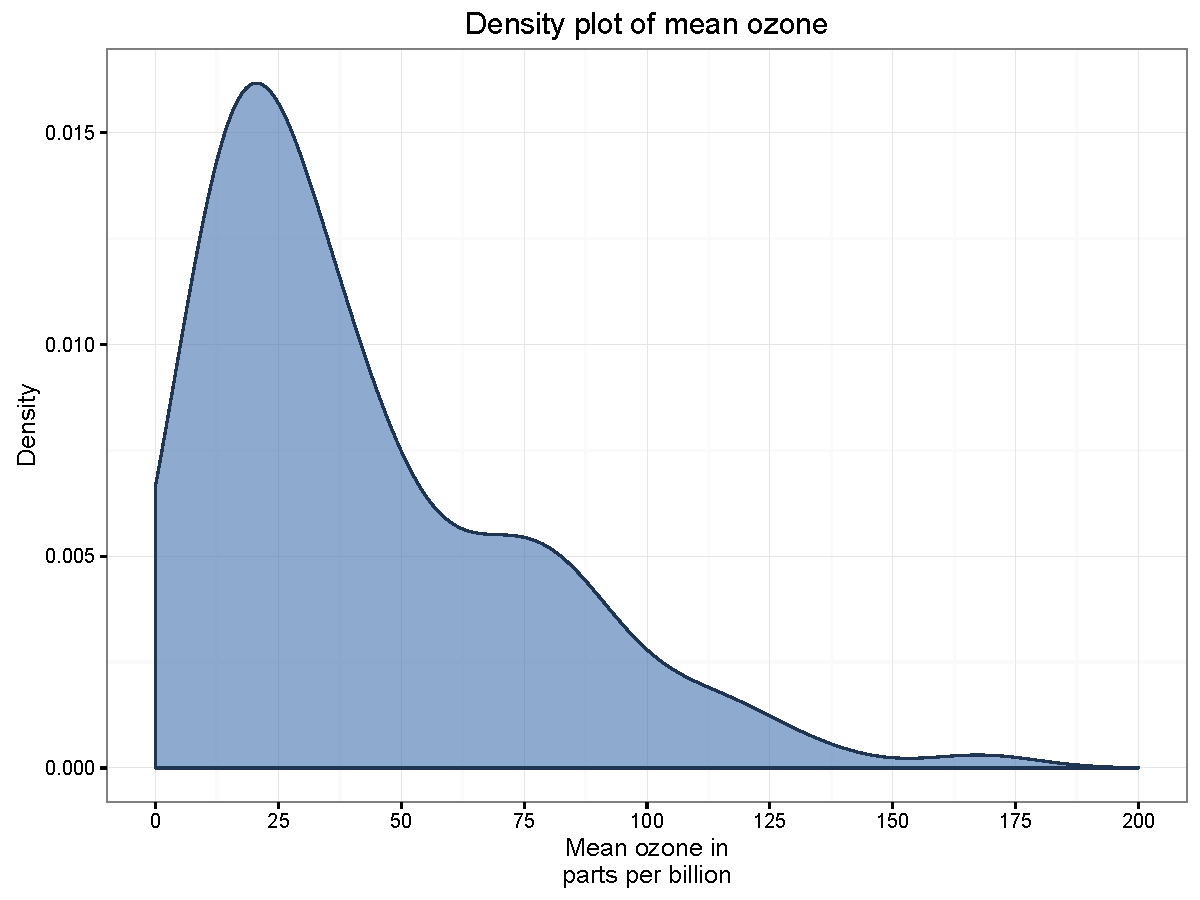
\includegraphics[width=0.55\linewidth]{figures/density_9-1} \end{center}

\section{Creating an XKCD style
chart}\label{creating-an-xkcd-style-chart-7}

Of course, you may want to create your own themes as well.
\texttt{ggplot2} allows for a very high degree of customisation,
including allowing you to use imported fonts. Below is an example of a
theme Mauricio was able to create which mimics the visual style of
\href{http://xkcd.com/}{XKCD}. In order to create this chart, you first
need to import the XKCD font, install it on your machine and load it
into R using the \texttt{extrafont} package. These instructions are
taken from
\href{https://www.google.com.au/url?sa=t\&rct=j\&q=\&esrc=s\&source=web\&cd=1\&ved=0ahUKEwiWzafchdPJAhVBpJQKHe_LDT8QFggbMAA\&url=https\%3A\%2F\%2Fcran.r-project.org\%2Fweb\%2Fpackages\%2Fxkcd\%2Fvignettes\%2Fxkcd-intro.pdf\&usg=AFQjCNE-KciGY14e-Q1buYIVmTFC0ht__Q\&sig2=DZUwkvIHwfNWtTtkcz94jg}{here}:

\begin{Shaded}
\begin{Highlighting}[]
\KeywordTok{library}\NormalTok{(extrafont)}

\KeywordTok{download.file}\NormalTok{(}\StringTok{"http://simonsoftware.se/other/xkcd.ttf"}\NormalTok{, }
\StringTok{      }\DataTypeTok{dest=}\StringTok{"xkcd.ttf"}\NormalTok{, }\DataTypeTok{mode=}\StringTok{"wb"}\NormalTok{)}
\KeywordTok{system}\NormalTok{(}\StringTok{"mkdir ~/.fonts"}\NormalTok{)}
\KeywordTok{system}\NormalTok{(}\StringTok{"cp xkcd.ttf  ~/.fonts"}\NormalTok{)}
\KeywordTok{font_import}\NormalTok{(}\DataTypeTok{paths =} \StringTok{"~/.fonts"}\NormalTok{, }\DataTypeTok{pattern=}\StringTok{"[X/x]kcd"}\NormalTok{)}
\KeywordTok{fonts}\NormalTok{()}
\KeywordTok{loadfonts}\NormalTok{()}
\end{Highlighting}
\end{Shaded}

You can then create your graph:

\begin{Shaded}
\begin{Highlighting}[]
\NormalTok{p8 <-}\StringTok{ }\KeywordTok{ggplot}\NormalTok{(airquality, }\KeywordTok{aes}\NormalTok{(}\DataTypeTok{x =} \NormalTok{Ozone)) +}\StringTok{ }
\StringTok{      }\KeywordTok{geom_density}\NormalTok{(}\DataTypeTok{colour =} \StringTok{"black"}\NormalTok{, }\DataTypeTok{fill =} \StringTok{"#56B4E9"}\NormalTok{) +}
\StringTok{      }\KeywordTok{scale_x_continuous}\NormalTok{(}\DataTypeTok{name =} \StringTok{"Mean ozone in}\CharTok{\textbackslash{}n}\StringTok{parts per billion"}\NormalTok{,}
\StringTok{        }\DataTypeTok{breaks =} \KeywordTok{seq}\NormalTok{(}\DecValTok{0}\NormalTok{, }\DecValTok{200}\NormalTok{, }\DecValTok{25}\NormalTok{),}
\StringTok{        }\DataTypeTok{limits=}\KeywordTok{c}\NormalTok{(}\DecValTok{0}\NormalTok{, }\DecValTok{200}\NormalTok{)) +}
\StringTok{      }\KeywordTok{scale_y_continuous}\NormalTok{(}\DataTypeTok{name =} \StringTok{"Density"}\NormalTok{) +}
\StringTok{      }\KeywordTok{ggtitle}\NormalTok{(}\StringTok{"Density plot of mean ozone"}\NormalTok{) +}
\StringTok{      }\KeywordTok{theme}\NormalTok{(}\DataTypeTok{axis.line.x =} \KeywordTok{element_line}\NormalTok{(}\DataTypeTok{size=}\NormalTok{.}\DecValTok{5}\NormalTok{, }\DataTypeTok{colour =} \StringTok{"black"}\NormalTok{),}
\StringTok{        }\DataTypeTok{axis.line.y =} \KeywordTok{element_line}\NormalTok{(}\DataTypeTok{size=}\NormalTok{.}\DecValTok{5}\NormalTok{, }\DataTypeTok{colour =} \StringTok{"black"}\NormalTok{), }
\StringTok{        }\DataTypeTok{axis.text.x=}\KeywordTok{element_text}\NormalTok{(}\DataTypeTok{colour=}\StringTok{"black"}\NormalTok{, }\DataTypeTok{size =} \DecValTok{9}\NormalTok{), }
\StringTok{        }\DataTypeTok{axis.text.y=}\KeywordTok{element_text}\NormalTok{(}\DataTypeTok{colour=}\StringTok{"black"}\NormalTok{, }\DataTypeTok{size =} \DecValTok{9}\NormalTok{),}
\StringTok{        }\DataTypeTok{panel.grid.major =} \KeywordTok{element_line}\NormalTok{(}\DataTypeTok{colour =} \StringTok{"#d3d3d3"}\NormalTok{), }
\StringTok{        }\DataTypeTok{panel.grid.minor =} \KeywordTok{element_blank}\NormalTok{(), }
\StringTok{        }\DataTypeTok{panel.border =} \KeywordTok{element_blank}\NormalTok{(), }\DataTypeTok{panel.background =} \KeywordTok{element_blank}\NormalTok{(),}
\StringTok{        }\DataTypeTok{plot.title =} \KeywordTok{element_text}\NormalTok{(}\DataTypeTok{family =} \StringTok{"xkcd-Regular"}\NormalTok{),}
\StringTok{        }\DataTypeTok{text=}\KeywordTok{element_text}\NormalTok{(}\DataTypeTok{family=}\StringTok{"xkcd-Regular"}\NormalTok{))}
\NormalTok{p8}
\end{Highlighting}
\end{Shaded}

\begin{center}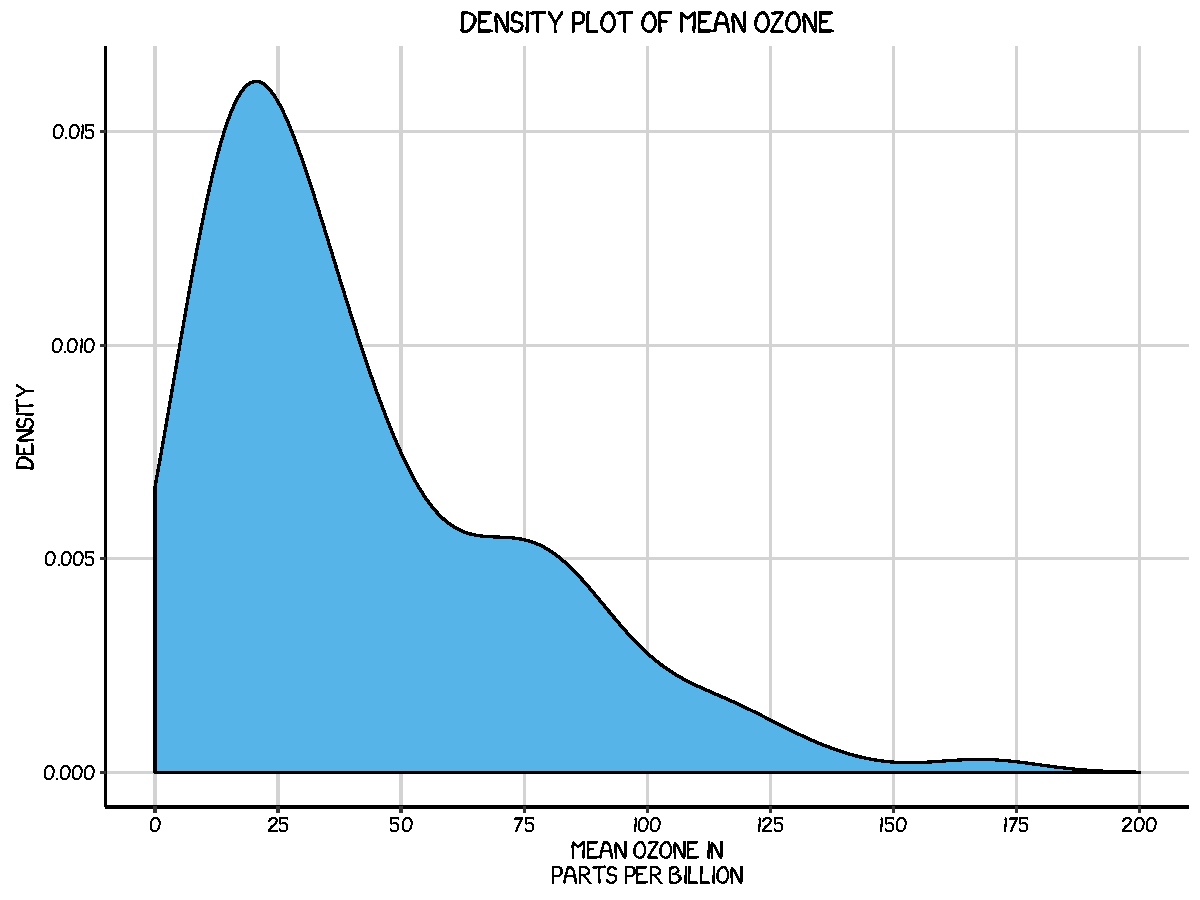
\includegraphics[width=0.55\linewidth]{figures/density_10-1} \end{center}

\section{\texorpdfstring{Using `The Economist'
theme}{Using The Economist theme}}\label{using-the-economist-theme-7}

There are a wider range of pre-built themes available as part of the
\texttt{ggthemes} package (more information on these
\href{https://cran.r-project.org/web/packages/ggthemes/vignettes/ggthemes.html}{here}).
Below we've applied \texttt{theme\_economist()}, which approximates
graphs in the Economist magazine.

\begin{Shaded}
\begin{Highlighting}[]
\KeywordTok{library}\NormalTok{(ggthemes)}
\KeywordTok{library}\NormalTok{(grid)}

\NormalTok{fill <-}\StringTok{ "#4271AE"}
\NormalTok{line <-}\StringTok{ "#1F3552"}

\NormalTok{p8 <-}\StringTok{ }\KeywordTok{ggplot}\NormalTok{(airquality, }\KeywordTok{aes}\NormalTok{(}\DataTypeTok{x =} \NormalTok{Ozone)) +}\StringTok{ }
\StringTok{      }\KeywordTok{geom_density}\NormalTok{(}\DataTypeTok{fill =} \NormalTok{fill, }\DataTypeTok{colour =} \NormalTok{line) +}
\StringTok{      }\KeywordTok{scale_x_continuous}\NormalTok{(}\DataTypeTok{name =} \StringTok{"Mean ozone in}\CharTok{\textbackslash{}n}\StringTok{parts per billion"}\NormalTok{,}
\StringTok{        }\DataTypeTok{breaks =} \KeywordTok{seq}\NormalTok{(}\DecValTok{0}\NormalTok{, }\DecValTok{200}\NormalTok{, }\DecValTok{25}\NormalTok{),}
\StringTok{        }\DataTypeTok{limits=}\KeywordTok{c}\NormalTok{(}\DecValTok{0}\NormalTok{, }\DecValTok{200}\NormalTok{)) +}
\StringTok{      }\KeywordTok{scale_y_continuous}\NormalTok{(}\DataTypeTok{name =} \StringTok{"Density"}\NormalTok{) +}
\StringTok{      }\KeywordTok{ggtitle}\NormalTok{(}\StringTok{"Density plot of mean ozone"}\NormalTok{) +}
\StringTok{      }\KeywordTok{theme_economist}\NormalTok{() +}
\StringTok{      }\KeywordTok{theme}\NormalTok{(}\DataTypeTok{axis.line.x =} \KeywordTok{element_line}\NormalTok{(}\DataTypeTok{size=}\NormalTok{.}\DecValTok{5}\NormalTok{, }\DataTypeTok{colour =} \StringTok{"black"}\NormalTok{),}
\StringTok{        }\DataTypeTok{axis.line.y =} \KeywordTok{element_line}\NormalTok{(}\DataTypeTok{size=}\NormalTok{.}\DecValTok{5}\NormalTok{, }\DataTypeTok{colour =} \StringTok{"black"}\NormalTok{), }
\StringTok{        }\DataTypeTok{axis.text.x=}\KeywordTok{element_text}\NormalTok{(}\DataTypeTok{colour=}\StringTok{"black"}\NormalTok{, }\DataTypeTok{size =} \DecValTok{9}\NormalTok{), }
\StringTok{        }\DataTypeTok{axis.text.y=}\KeywordTok{element_text}\NormalTok{(}\DataTypeTok{colour=}\StringTok{"black"}\NormalTok{, }\DataTypeTok{size =} \DecValTok{9}\NormalTok{),}
\StringTok{        }\DataTypeTok{panel.grid.major =} \KeywordTok{element_line}\NormalTok{(}\DataTypeTok{colour =} \StringTok{"#d3d3d3"}\NormalTok{), }
\StringTok{        }\DataTypeTok{panel.grid.minor =} \KeywordTok{element_blank}\NormalTok{(), }
\StringTok{        }\DataTypeTok{panel.border =} \KeywordTok{element_blank}\NormalTok{(), }\DataTypeTok{panel.background =} \KeywordTok{element_blank}\NormalTok{(),}
\StringTok{        }\DataTypeTok{plot.title =} \KeywordTok{element_text}\NormalTok{(}\DataTypeTok{family =} \StringTok{"OfficinaSanITC-Book"}\NormalTok{),}
\StringTok{        }\DataTypeTok{text=}\KeywordTok{element_text}\NormalTok{(}\DataTypeTok{family=}\StringTok{"OfficinaSanITC-Book"}\NormalTok{))}
\NormalTok{p8}
\end{Highlighting}
\end{Shaded}

\begin{center}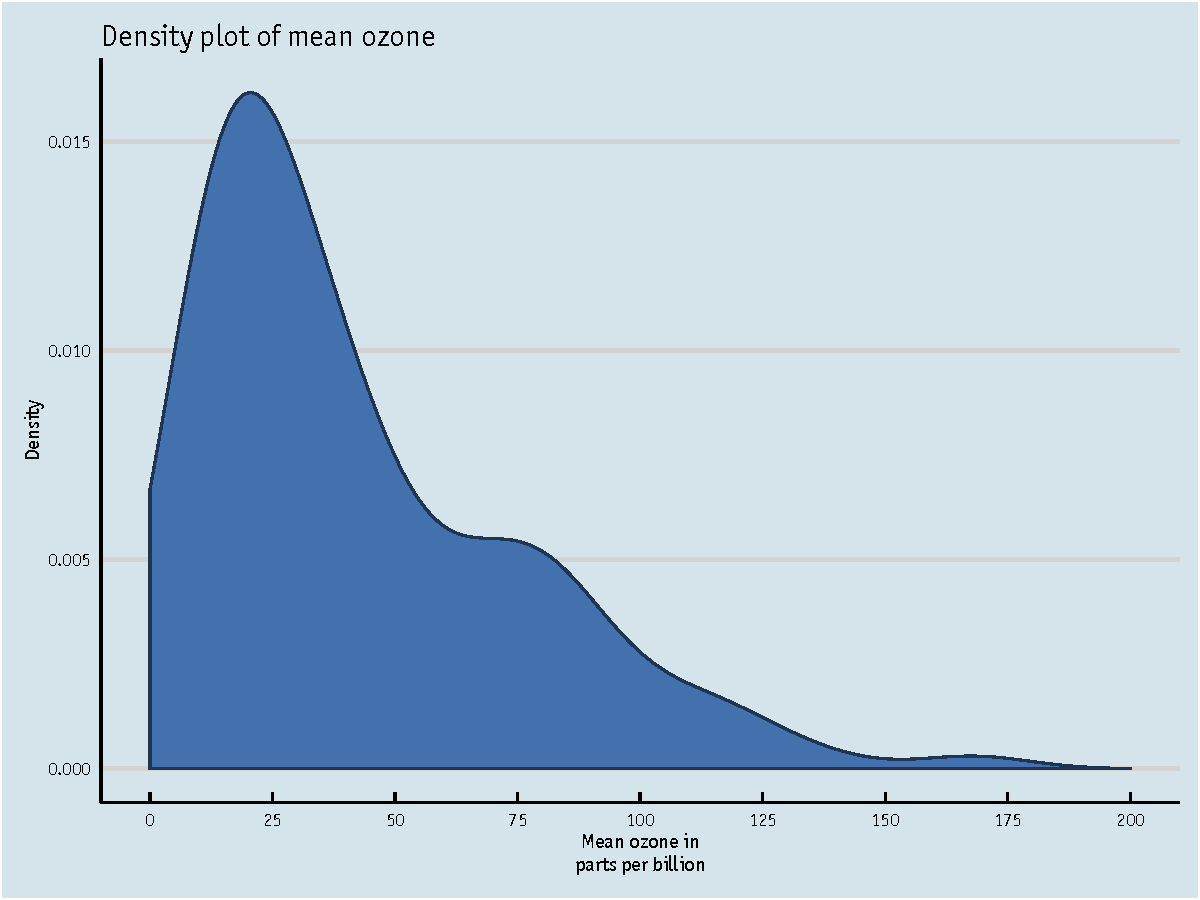
\includegraphics[width=0.55\linewidth]{figures/density_11-1} \end{center}

\section{Creating your own theme}\label{creating-your-own-theme-7}

As before, you can modify your plots a lot as \texttt{ggplot2} allows
many customisations. Here is a custom plot where we have modified the
axes, background and font.

\begin{Shaded}
\begin{Highlighting}[]
\KeywordTok{library}\NormalTok{(grid) }

\NormalTok{fill <-}\StringTok{ "#4271AE"}
\NormalTok{lines <-}\StringTok{ "#1F3552"}

\NormalTok{p8 <-}\StringTok{ }\KeywordTok{ggplot}\NormalTok{(airquality, }\KeywordTok{aes}\NormalTok{(}\DataTypeTok{x =} \NormalTok{Ozone)) +}\StringTok{ }
\StringTok{      }\KeywordTok{geom_density}\NormalTok{(}\DataTypeTok{colour =} \NormalTok{lines, }\DataTypeTok{fill =} \NormalTok{fill, }\DataTypeTok{size =} \DecValTok{1}\NormalTok{) +}
\StringTok{      }\KeywordTok{scale_x_continuous}\NormalTok{(}\DataTypeTok{name =} \StringTok{"Mean ozone in}\CharTok{\textbackslash{}n}\StringTok{parts per billion"}\NormalTok{,}
\StringTok{        }\DataTypeTok{breaks =} \KeywordTok{seq}\NormalTok{(}\DecValTok{0}\NormalTok{, }\DecValTok{200}\NormalTok{, }\DecValTok{25}\NormalTok{),}
\StringTok{        }\DataTypeTok{limits=}\KeywordTok{c}\NormalTok{(}\DecValTok{0}\NormalTok{, }\DecValTok{200}\NormalTok{)) +}
\StringTok{      }\KeywordTok{scale_y_continuous}\NormalTok{(}\DataTypeTok{name =} \StringTok{"Density"}\NormalTok{) +}
\StringTok{      }\KeywordTok{ggtitle}\NormalTok{(}\StringTok{"Density plot of mean ozone"}\NormalTok{) +}
\StringTok{      }\KeywordTok{theme}\NormalTok{(}\DataTypeTok{axis.line.x =} \KeywordTok{element_line}\NormalTok{(}\DataTypeTok{size=}\NormalTok{.}\DecValTok{5}\NormalTok{, }\DataTypeTok{colour =} \StringTok{"black"}\NormalTok{),}
\StringTok{        }\DataTypeTok{axis.line.y =} \KeywordTok{element_line}\NormalTok{(}\DataTypeTok{size=}\NormalTok{.}\DecValTok{5}\NormalTok{, }\DataTypeTok{colour =} \StringTok{"black"}\NormalTok{),}
\StringTok{        }\DataTypeTok{axis.text.x=}\KeywordTok{element_text}\NormalTok{(}\DataTypeTok{colour=}\StringTok{"black"}\NormalTok{, }\DataTypeTok{size =} \DecValTok{9}\NormalTok{), }
\StringTok{        }\DataTypeTok{axis.text.y=}\KeywordTok{element_text}\NormalTok{(}\DataTypeTok{colour=}\StringTok{"black"}\NormalTok{, }\DataTypeTok{size =} \DecValTok{9}\NormalTok{), }
\StringTok{        }\DataTypeTok{legend.position =} \StringTok{"bottom"}\NormalTok{, }\DataTypeTok{legend.position =} \StringTok{"horizontal"}\NormalTok{,}
\StringTok{        }\DataTypeTok{panel.grid.major =} \KeywordTok{element_line}\NormalTok{(}\DataTypeTok{colour =} \StringTok{"#d3d3d3"}\NormalTok{), }
\StringTok{        }\DataTypeTok{panel.grid.minor =} \KeywordTok{element_blank}\NormalTok{(), }
\StringTok{        }\DataTypeTok{panel.border =} \KeywordTok{element_blank}\NormalTok{(), }\DataTypeTok{panel.background =} \KeywordTok{element_blank}\NormalTok{(),}
\StringTok{        }\DataTypeTok{plot.title =} \KeywordTok{element_text}\NormalTok{(}\DataTypeTok{size =} \DecValTok{14}\NormalTok{, }\DataTypeTok{family =} \StringTok{"Tahoma"}\NormalTok{, }\DataTypeTok{face =} \StringTok{"bold"}\NormalTok{),}
\StringTok{        }\DataTypeTok{text=}\KeywordTok{element_text}\NormalTok{(}\DataTypeTok{family=}\StringTok{"Tahoma"}\NormalTok{))}
\NormalTok{p8}
\end{Highlighting}
\end{Shaded}

\begin{center}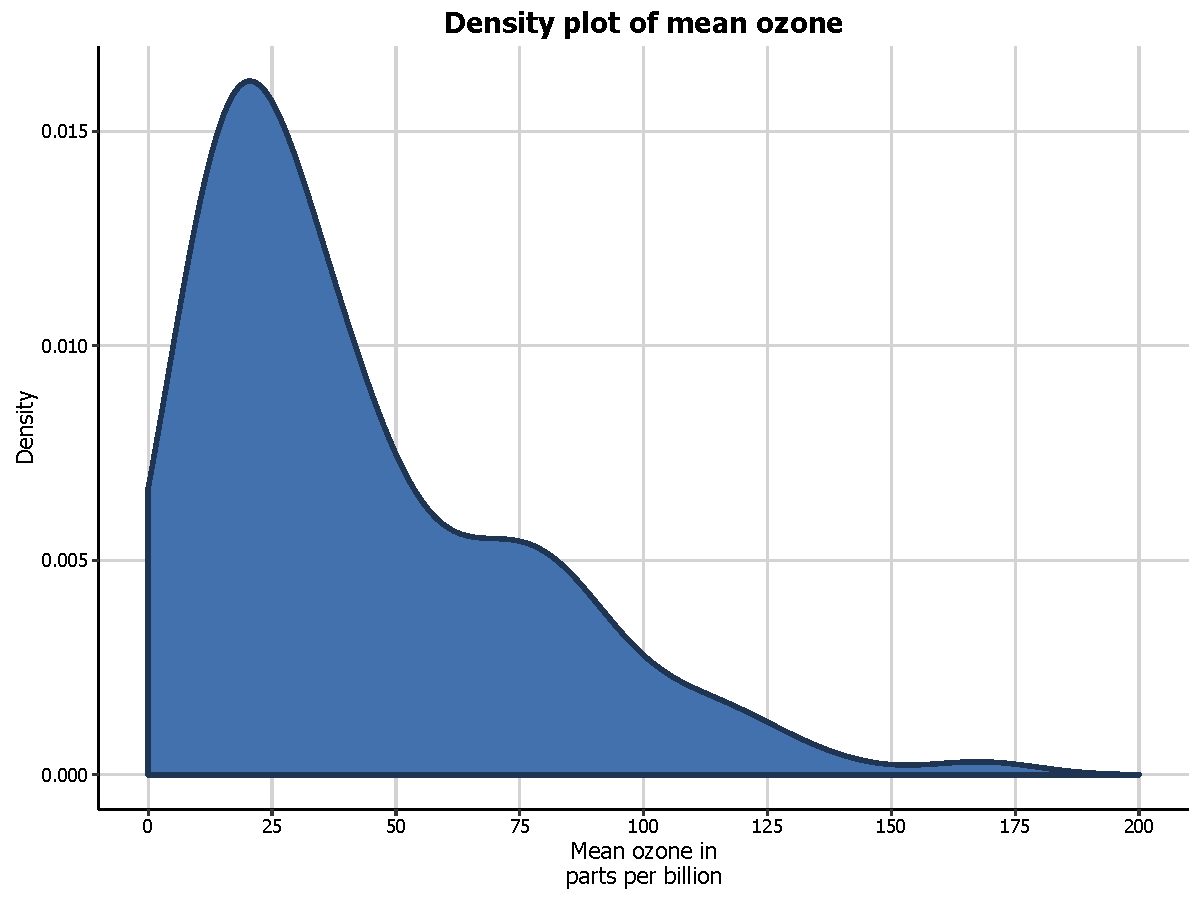
\includegraphics[width=0.55\linewidth]{figures/density_12-1} \end{center}

\section{Adding lines}\label{adding-lines-1}

Let's say that we want to add a cutoff value to the chart (75 parts of
ozone per billion). We add the \texttt{geom\_vline} option to the chart,
and specify where it goes on the x-axis using the \texttt{xintercept}
argument. We can customise how it looks using the \texttt{colour} and
\texttt{linetype} arguments in \texttt{geom\_vline}. (In the the same
way, horizontal lines can be added using the \texttt{geom\_hline}.)

\begin{Shaded}
\begin{Highlighting}[]
\NormalTok{fill <-}\StringTok{ "#4271AE"}
\NormalTok{line <-}\StringTok{ "#1F3552"}

\NormalTok{p8 <-}\StringTok{ }\NormalTok{p8 +}\StringTok{ }\KeywordTok{geom_vline}\NormalTok{(}\DataTypeTok{xintercept =} \DecValTok{75}\NormalTok{, }\DataTypeTok{size =} \DecValTok{1}\NormalTok{, }\DataTypeTok{colour =} \StringTok{"#FF3721"}\NormalTok{, }
\StringTok{        }\DataTypeTok{linetype =} \StringTok{"dashed"}\NormalTok{)}
\NormalTok{p8}
\end{Highlighting}
\end{Shaded}

\begin{center}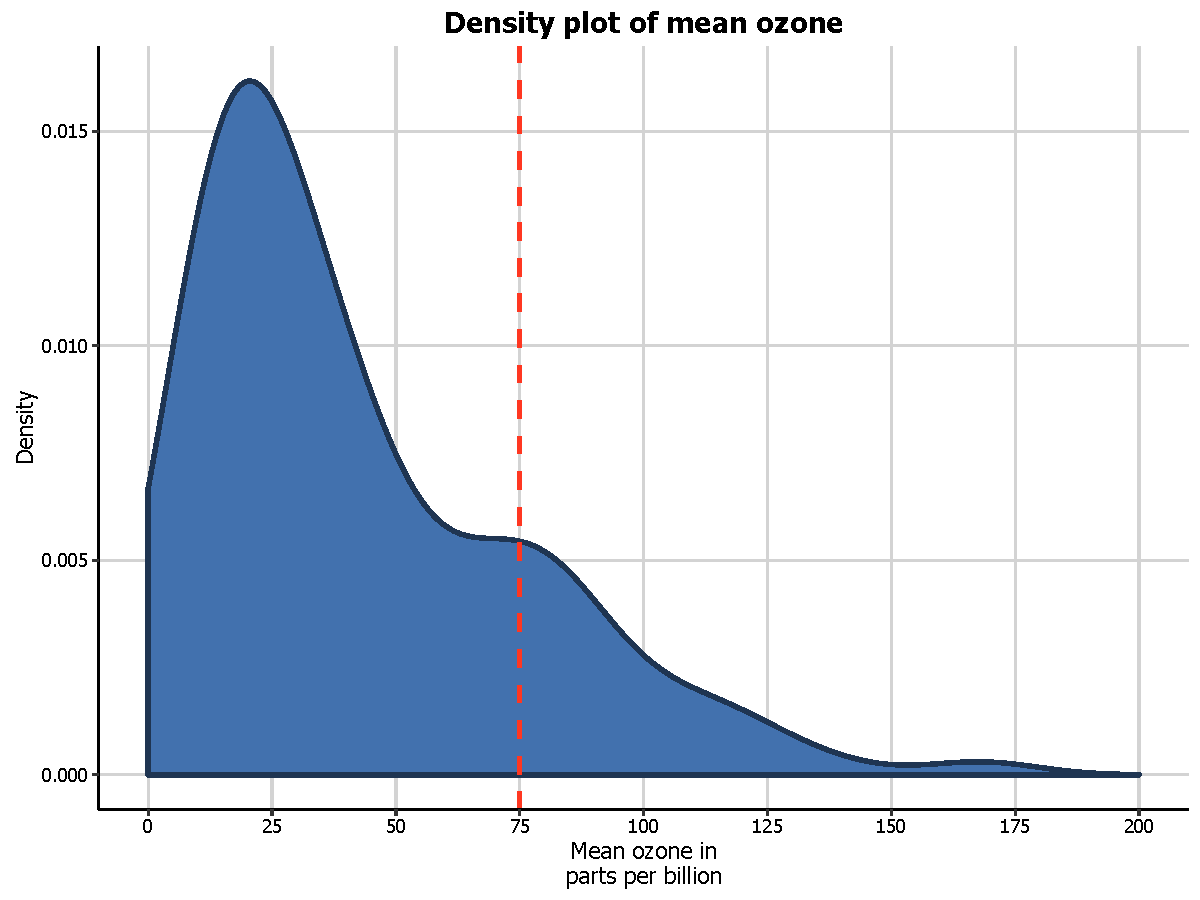
\includegraphics[width=0.55\linewidth]{figures/density_13-1} \end{center}

\section{Multiple densities}\label{multiple-densities}

You can also easily create multiple density plots by the levels of
another variable. There are two options, in separate (panel) plots, or
in the same plot. There are also a couple of variations on these we'll
discuss below.

We first need to do a little data wrangling. In order to make the graphs
a bit clearer, we've kept only months ``5'' (May), ``6'' (June) and
``7'' (July) in a new dataset \texttt{airquality\_trimmed}. We also need
to convert this variable into either a character or factor variable. We
have created a new factor variable \texttt{Month.f}.

In order to produce a panel plot by month, we add the
\texttt{facet\_grid(.\ \textasciitilde{}\ Month.f)} option to the plot.
Note that we've also changed the scale of the x-axis to make it fit a
little more neatly in the panel format.

\begin{Shaded}
\begin{Highlighting}[]
\NormalTok{airquality_trimmed <-}\StringTok{ }\NormalTok{airquality[}\KeywordTok{which}\NormalTok{(airquality$Month ==}\StringTok{ }\DecValTok{5} \NormalTok{|}
\StringTok{        }\NormalTok{airquality$Month ==}\StringTok{ }\DecValTok{6} \NormalTok{|}
\StringTok{        }\NormalTok{airquality$Month ==}\StringTok{ }\DecValTok{7}\NormalTok{), ]}
\NormalTok{airquality_trimmed$Month.f <-}\StringTok{ }\KeywordTok{factor}\NormalTok{(airquality_trimmed$Month, }
\StringTok{        }\DataTypeTok{labels =} \KeywordTok{c}\NormalTok{(}\StringTok{"May"}\NormalTok{, }\StringTok{"June"}\NormalTok{, }\StringTok{"July"}\NormalTok{))}

\NormalTok{p8 <-}\StringTok{ }\KeywordTok{ggplot}\NormalTok{(airquality_trimmed, }\KeywordTok{aes}\NormalTok{(}\DataTypeTok{x =} \NormalTok{Ozone)) +}\StringTok{ }
\StringTok{      }\KeywordTok{geom_density}\NormalTok{(}\DataTypeTok{fill =} \NormalTok{fill, }\DataTypeTok{colour =} \NormalTok{line,}
\StringTok{        }\DataTypeTok{alpha =} \FloatTok{0.6}\NormalTok{) +}
\StringTok{      }\KeywordTok{scale_x_continuous}\NormalTok{(}\DataTypeTok{name =} \StringTok{"Mean ozone in}\CharTok{\textbackslash{}n}\StringTok{parts per billion"}\NormalTok{,}
\StringTok{        }\DataTypeTok{breaks =} \KeywordTok{seq}\NormalTok{(}\DecValTok{0}\NormalTok{, }\DecValTok{200}\NormalTok{, }\DecValTok{50}\NormalTok{),}
\StringTok{        }\DataTypeTok{limits=}\KeywordTok{c}\NormalTok{(}\DecValTok{0}\NormalTok{, }\DecValTok{200}\NormalTok{)) +}
\StringTok{      }\KeywordTok{scale_y_continuous}\NormalTok{(}\DataTypeTok{name =} \StringTok{"Density"}\NormalTok{) +}
\StringTok{      }\KeywordTok{ggtitle}\NormalTok{(}\StringTok{"Density plot of mean ozone"}\NormalTok{) +}
\StringTok{      }\KeywordTok{facet_grid}\NormalTok{(. ~}\StringTok{ }\NormalTok{Month.f) +}
\StringTok{      }\KeywordTok{theme_bw}\NormalTok{() +}
\StringTok{      }\KeywordTok{theme}\NormalTok{(}\DataTypeTok{plot.title =} \KeywordTok{element_text}\NormalTok{(}\DataTypeTok{size =} \DecValTok{14}\NormalTok{, }\DataTypeTok{family =} \StringTok{"Tahoma"}\NormalTok{, }\DataTypeTok{face =} \StringTok{"bold"}\NormalTok{), }
\StringTok{        }\DataTypeTok{text =} \KeywordTok{element_text}\NormalTok{(}\DataTypeTok{size =} \DecValTok{12}\NormalTok{, }\DataTypeTok{family =} \StringTok{"Tahoma"}\NormalTok{))}
\NormalTok{p8}
\end{Highlighting}
\end{Shaded}

\begin{center}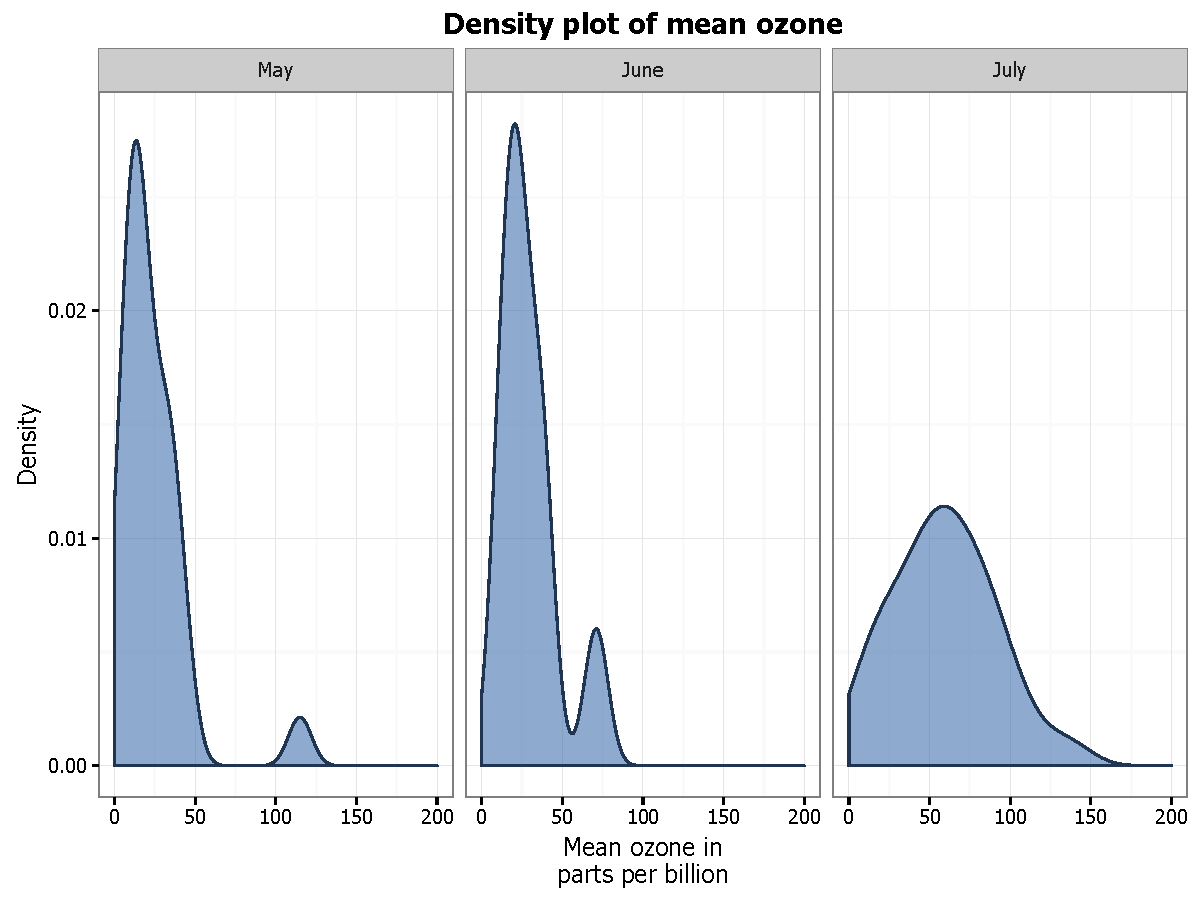
\includegraphics[width=0.55\linewidth]{figures/density_14-1} \end{center}

An alternative to a panel plot is the \emph{volcano plot}. This plot
swaps the axes (so the variable of interest is on the y-axis and the
density is on the x-axis), and reflects the density. In order to create
this plot, we replace \texttt{geom\_density} with
\texttt{stat\_density}, and include the arguments
\texttt{aes(ymax\ =\ ..density..,\ \ ymin\ =\ -..density..)} and
\texttt{geom\ =\ \"ribbon\"} to create a density plot, the usual
\texttt{fill}, \texttt{colour} and \texttt{alpha} arguments, and
\texttt{position\ =\ \"identity\"}. We also need to add a
\texttt{coord\_flip()} option to the plot.

\begin{Shaded}
\begin{Highlighting}[]
\NormalTok{p8 <-}\StringTok{ }\KeywordTok{ggplot}\NormalTok{(airquality_trimmed, }\KeywordTok{aes}\NormalTok{(}\DataTypeTok{x =} \NormalTok{Ozone)) +}\StringTok{ }
\StringTok{      }\KeywordTok{stat_density}\NormalTok{(}\KeywordTok{aes}\NormalTok{(}\DataTypeTok{ymax =} \NormalTok{..density..,  }\DataTypeTok{ymin =} \NormalTok{-..density..),}
\StringTok{        }\DataTypeTok{geom =} \StringTok{"ribbon"}\NormalTok{, }
\StringTok{        }\DataTypeTok{fill =} \NormalTok{fill, }\DataTypeTok{colour =} \NormalTok{line, }\DataTypeTok{alpha =} \FloatTok{0.6}\NormalTok{,}
\StringTok{        }\DataTypeTok{position =} \StringTok{"identity"}\NormalTok{) +}
\StringTok{      }\KeywordTok{scale_x_continuous}\NormalTok{(}\DataTypeTok{name =} \StringTok{"Mean ozone in}\CharTok{\textbackslash{}n}\StringTok{parts per billion"}\NormalTok{,}
\StringTok{        }\DataTypeTok{breaks =} \KeywordTok{seq}\NormalTok{(}\DecValTok{0}\NormalTok{, }\DecValTok{200}\NormalTok{, }\DecValTok{25}\NormalTok{),}
\StringTok{        }\DataTypeTok{limits=}\KeywordTok{c}\NormalTok{(}\DecValTok{0}\NormalTok{, }\DecValTok{200}\NormalTok{)) +}
\StringTok{      }\KeywordTok{scale_y_continuous}\NormalTok{(}\DataTypeTok{name =} \StringTok{"Density"}\NormalTok{,}
\StringTok{        }\DataTypeTok{breaks =} \KeywordTok{seq}\NormalTok{(-}\FloatTok{0.03}\NormalTok{, }\FloatTok{0.03}\NormalTok{, }\FloatTok{0.03}\NormalTok{)) +}
\StringTok{      }\KeywordTok{ggtitle}\NormalTok{(}\StringTok{"Density plot of mean ozone"}\NormalTok{) +}
\StringTok{      }\KeywordTok{facet_grid}\NormalTok{(. ~}\StringTok{ }\NormalTok{Month.f) +}
\StringTok{      }\KeywordTok{coord_flip}\NormalTok{() +}
\StringTok{      }\KeywordTok{theme_bw}\NormalTok{() +}
\StringTok{      }\KeywordTok{theme}\NormalTok{(}\DataTypeTok{plot.title =} \KeywordTok{element_text}\NormalTok{(}\DataTypeTok{size =} \DecValTok{14}\NormalTok{, }\DataTypeTok{family =} \StringTok{"Tahoma"}\NormalTok{, }\DataTypeTok{face =} \StringTok{"bold"}\NormalTok{), }
\StringTok{        }\DataTypeTok{text =} \KeywordTok{element_text}\NormalTok{(}\DataTypeTok{size =} \DecValTok{12}\NormalTok{, }\DataTypeTok{family =} \StringTok{"Tahoma"}\NormalTok{))}
\NormalTok{p8}
\end{Highlighting}
\end{Shaded}

\begin{center}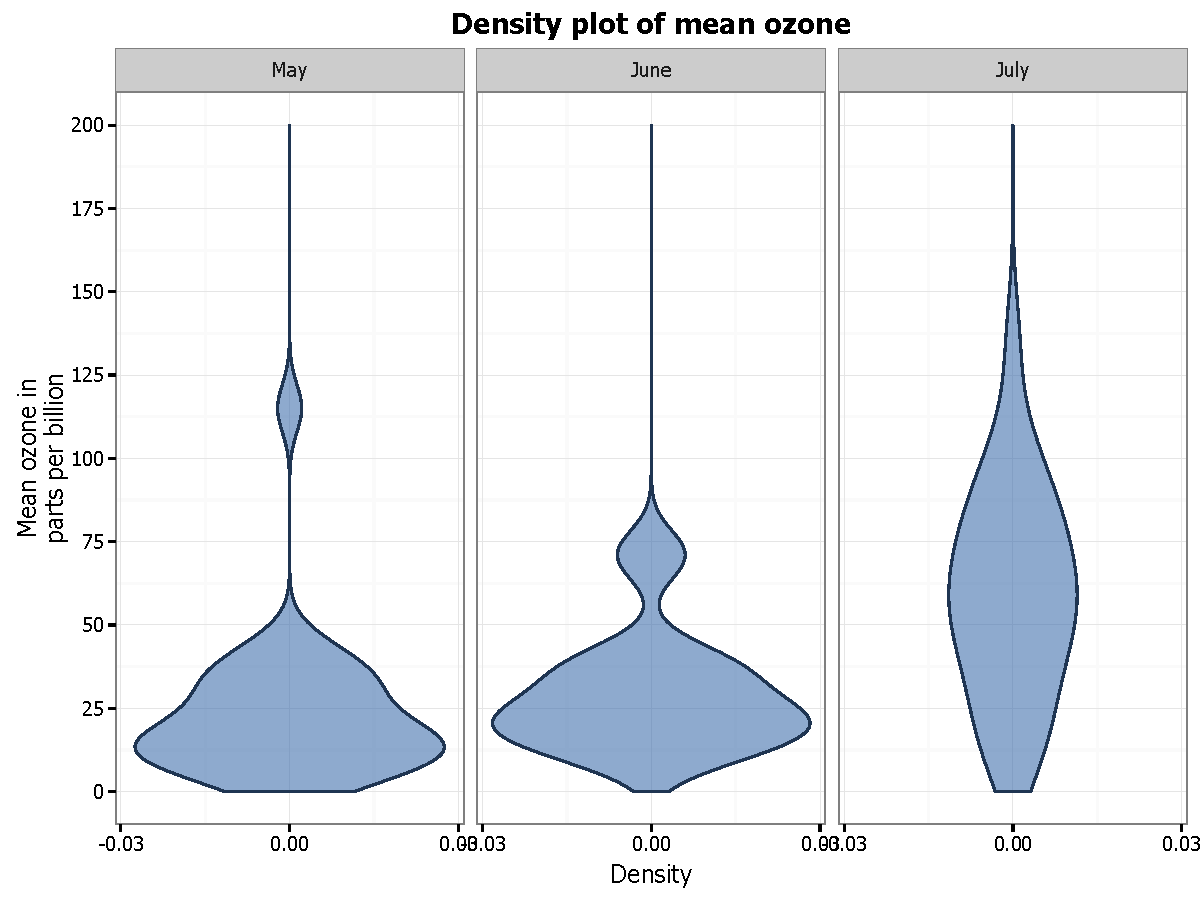
\includegraphics[width=0.55\linewidth]{figures/density_15-1} \end{center}

In order to plot the three months in the same plot, we add several
things. Firstly, in the \texttt{ggplot} function, we add a
\texttt{fill\ =\ Month.f} argument to \texttt{aes}. Secondly, in order
to more clearly see the graph, we add the argument
\texttt{position\ =\ "identity"} to the \texttt{geom\_density} option.
This controls the position of the curves respectively. Finally, you can
customise the colours of the histograms by adding the
\texttt{scale\_fill\_brewer} to the plot from the \texttt{RColorBrewer}
package.
\href{http://moderndata.plot.ly/create-colorful-graphs-in-r-with-rcolorbrewer-and-plotly/}{This}
blog post describes the available packages.

\begin{Shaded}
\begin{Highlighting}[]
\KeywordTok{library}\NormalTok{(RColorBrewer)}

\NormalTok{p8 <-}\StringTok{ }\KeywordTok{ggplot}\NormalTok{(airquality_trimmed, }\KeywordTok{aes}\NormalTok{(}\DataTypeTok{x =} \NormalTok{Ozone, }\DataTypeTok{fill =} \NormalTok{Month.f)) +}\StringTok{ }
\StringTok{      }\KeywordTok{geom_density}\NormalTok{(}\DataTypeTok{position=}\StringTok{"identity"}\NormalTok{, }\DataTypeTok{alpha=}\FloatTok{0.6}\NormalTok{) +}
\StringTok{      }\KeywordTok{scale_x_continuous}\NormalTok{(}\DataTypeTok{name =} \StringTok{"Mean ozone in}\CharTok{\textbackslash{}n}\StringTok{parts per billion"}\NormalTok{,}
\StringTok{        }\DataTypeTok{breaks =} \KeywordTok{seq}\NormalTok{(}\DecValTok{0}\NormalTok{, }\DecValTok{200}\NormalTok{, }\DecValTok{25}\NormalTok{),}
\StringTok{        }\DataTypeTok{limits=}\KeywordTok{c}\NormalTok{(}\DecValTok{0}\NormalTok{, }\DecValTok{200}\NormalTok{)) +}
\StringTok{      }\KeywordTok{scale_y_continuous}\NormalTok{(}\DataTypeTok{name =} \StringTok{"Density"}\NormalTok{) +}
\StringTok{      }\KeywordTok{ggtitle}\NormalTok{(}\StringTok{"Density plot of mean ozone"}\NormalTok{) +}
\StringTok{      }\KeywordTok{scale_fill_brewer}\NormalTok{(}\DataTypeTok{palette=}\StringTok{"Accent"}\NormalTok{) +}
\StringTok{      }\KeywordTok{theme_bw}\NormalTok{() +}
\StringTok{      }\KeywordTok{theme}\NormalTok{(}\DataTypeTok{plot.title =} \KeywordTok{element_text}\NormalTok{(}\DataTypeTok{size =} \DecValTok{14}\NormalTok{, }\DataTypeTok{family =} \StringTok{"Tahoma"}\NormalTok{, }\DataTypeTok{face =} \StringTok{"bold"}\NormalTok{), }
\StringTok{        }\DataTypeTok{text =} \KeywordTok{element_text}\NormalTok{(}\DataTypeTok{size =} \DecValTok{12}\NormalTok{, }\DataTypeTok{family =} \StringTok{"Tahoma"}\NormalTok{))}
\NormalTok{p8}
\end{Highlighting}
\end{Shaded}

\begin{center}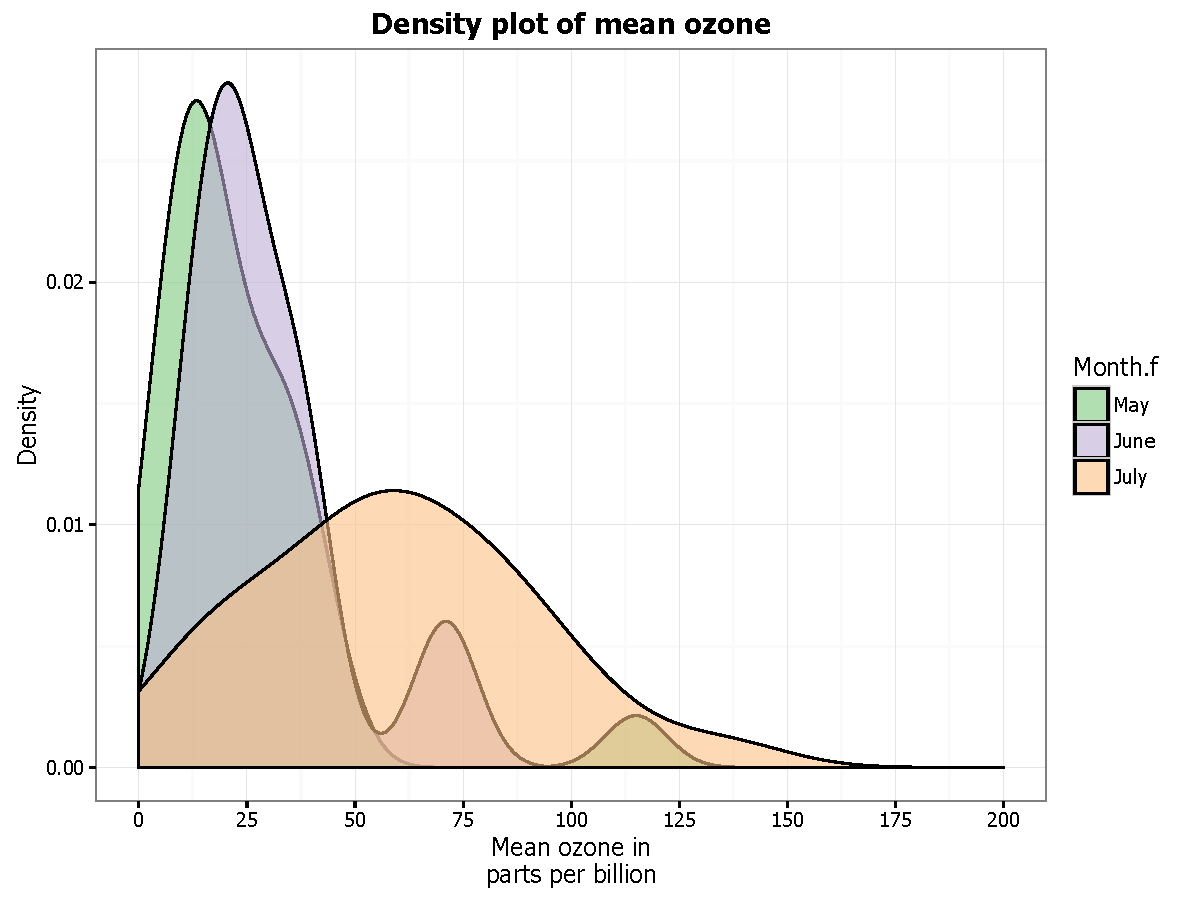
\includegraphics[width=0.55\linewidth]{figures/density_16-1} \end{center}

These densities are a little hard to see. One way we can make it easier
to see them is to stack the densities on top of each other. To do so, we
swap \texttt{position\ =\ "stack"} for \texttt{position\ =\ "identity"}
in \texttt{geom\_density}.

\begin{Shaded}
\begin{Highlighting}[]
\NormalTok{p8 <-}\StringTok{ }\KeywordTok{ggplot}\NormalTok{(airquality_trimmed, }\KeywordTok{aes}\NormalTok{(}\DataTypeTok{x =} \NormalTok{Ozone, }\DataTypeTok{fill =} \NormalTok{Month.f)) +}\StringTok{ }
\StringTok{      }\KeywordTok{geom_density}\NormalTok{(}\DataTypeTok{position =} \StringTok{"stack"}\NormalTok{, }\DataTypeTok{alpha =} \FloatTok{0.6}\NormalTok{) +}
\StringTok{      }\KeywordTok{scale_x_continuous}\NormalTok{(}\DataTypeTok{name =} \StringTok{"Mean ozone in}\CharTok{\textbackslash{}n}\StringTok{parts per billion"}\NormalTok{,}
\StringTok{        }\DataTypeTok{breaks =} \KeywordTok{seq}\NormalTok{(}\DecValTok{0}\NormalTok{, }\DecValTok{200}\NormalTok{, }\DecValTok{25}\NormalTok{),}
\StringTok{        }\DataTypeTok{limits=}\KeywordTok{c}\NormalTok{(}\DecValTok{0}\NormalTok{, }\DecValTok{200}\NormalTok{)) +}
\StringTok{      }\KeywordTok{scale_y_continuous}\NormalTok{(}\DataTypeTok{name =} \StringTok{"Density"}\NormalTok{) +}
\StringTok{      }\KeywordTok{ggtitle}\NormalTok{(}\StringTok{"Density plot of mean ozone"}\NormalTok{) +}
\StringTok{      }\KeywordTok{scale_fill_brewer}\NormalTok{(}\DataTypeTok{palette=}\StringTok{"Accent"}\NormalTok{) +}
\StringTok{      }\KeywordTok{theme_bw}\NormalTok{() +}
\StringTok{      }\KeywordTok{theme}\NormalTok{(}\DataTypeTok{plot.title =} \KeywordTok{element_text}\NormalTok{(}\DataTypeTok{size =} \DecValTok{14}\NormalTok{, }\DataTypeTok{family =} \StringTok{"Tahoma"}\NormalTok{, }\DataTypeTok{face =} \StringTok{"bold"}\NormalTok{), }
\StringTok{        }\DataTypeTok{text =} \KeywordTok{element_text}\NormalTok{(}\DataTypeTok{size =} \DecValTok{12}\NormalTok{, }\DataTypeTok{family =} \StringTok{"Tahoma"}\NormalTok{))}
\NormalTok{p8}
\end{Highlighting}
\end{Shaded}

\begin{center}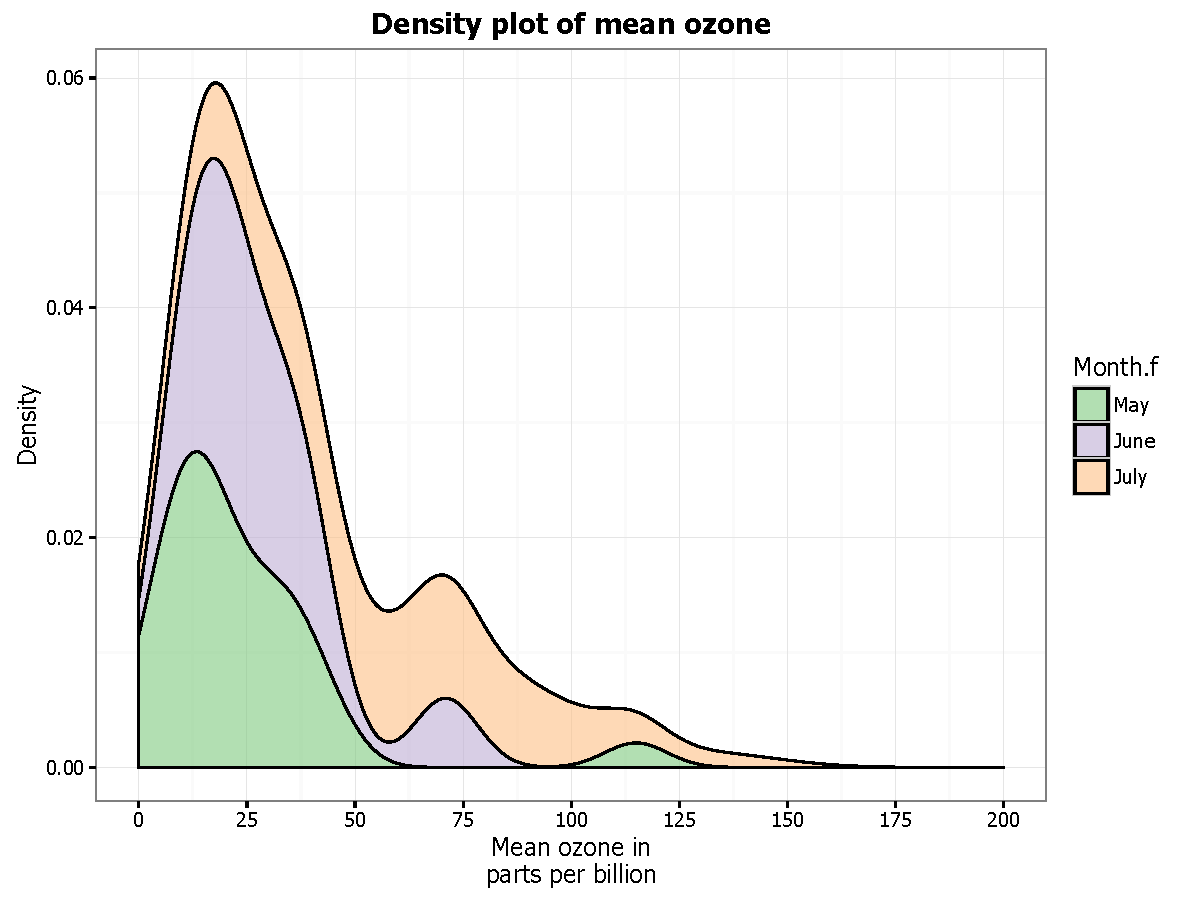
\includegraphics[width=0.55\linewidth]{figures/density_17-1} \end{center}

Another way to make it a little easier to see the densities by dropping
out the fill. To do this need a few changes. We need to swap the option
\texttt{fill\ =\ Month.f} in \texttt{ggplot} for
\texttt{colour\ =\ Month.f}. We add the \texttt{fill\ =\ NA} to
\texttt{geom\_density}, and we've also added \texttt{size\ =\ 1} to make
it easier to see the lines. Finally, we change the
\texttt{scale\_fill\_brewer()} option for
\texttt{scale\_colour\_brewer()}.

\begin{Shaded}
\begin{Highlighting}[]
\NormalTok{p8 <-}\StringTok{ }\KeywordTok{ggplot}\NormalTok{(airquality_trimmed, }\KeywordTok{aes}\NormalTok{(}\DataTypeTok{x =} \NormalTok{Ozone, }\DataTypeTok{colour =} \NormalTok{Month.f)) +}\StringTok{ }
\StringTok{      }\KeywordTok{geom_density}\NormalTok{(}\DataTypeTok{position=}\StringTok{"identity"}\NormalTok{, }\DataTypeTok{fill =} \OtherTok{NA}\NormalTok{, }\DataTypeTok{size =} \DecValTok{1}\NormalTok{) +}
\StringTok{      }\KeywordTok{scale_x_continuous}\NormalTok{(}\DataTypeTok{name =} \StringTok{"Mean ozone in}\CharTok{\textbackslash{}n}\StringTok{parts per billion"}\NormalTok{,}
\StringTok{        }\DataTypeTok{breaks =} \KeywordTok{seq}\NormalTok{(}\DecValTok{0}\NormalTok{, }\DecValTok{200}\NormalTok{, }\DecValTok{25}\NormalTok{),}
\StringTok{        }\DataTypeTok{limits=}\KeywordTok{c}\NormalTok{(}\DecValTok{0}\NormalTok{, }\DecValTok{200}\NormalTok{)) +}
\StringTok{      }\KeywordTok{scale_y_continuous}\NormalTok{(}\DataTypeTok{name =} \StringTok{"Density"}\NormalTok{) +}
\StringTok{      }\KeywordTok{ggtitle}\NormalTok{(}\StringTok{"Density plot of mean ozone"}\NormalTok{) +}
\StringTok{      }\KeywordTok{scale_colour_brewer}\NormalTok{(}\DataTypeTok{palette=}\StringTok{"Accent"}\NormalTok{) +}
\StringTok{      }\KeywordTok{theme_bw}\NormalTok{() +}
\StringTok{      }\KeywordTok{theme}\NormalTok{(}\DataTypeTok{plot.title =} \KeywordTok{element_text}\NormalTok{(}\DataTypeTok{size =} \DecValTok{14}\NormalTok{, }\DataTypeTok{family =} \StringTok{"Tahoma"}\NormalTok{, }\DataTypeTok{face =} \StringTok{"bold"}\NormalTok{), }
\StringTok{        }\DataTypeTok{text =} \KeywordTok{element_text}\NormalTok{(}\DataTypeTok{size =} \DecValTok{12}\NormalTok{, }\DataTypeTok{family =} \StringTok{"Tahoma"}\NormalTok{))}
\NormalTok{p8}
\end{Highlighting}
\end{Shaded}

\begin{center}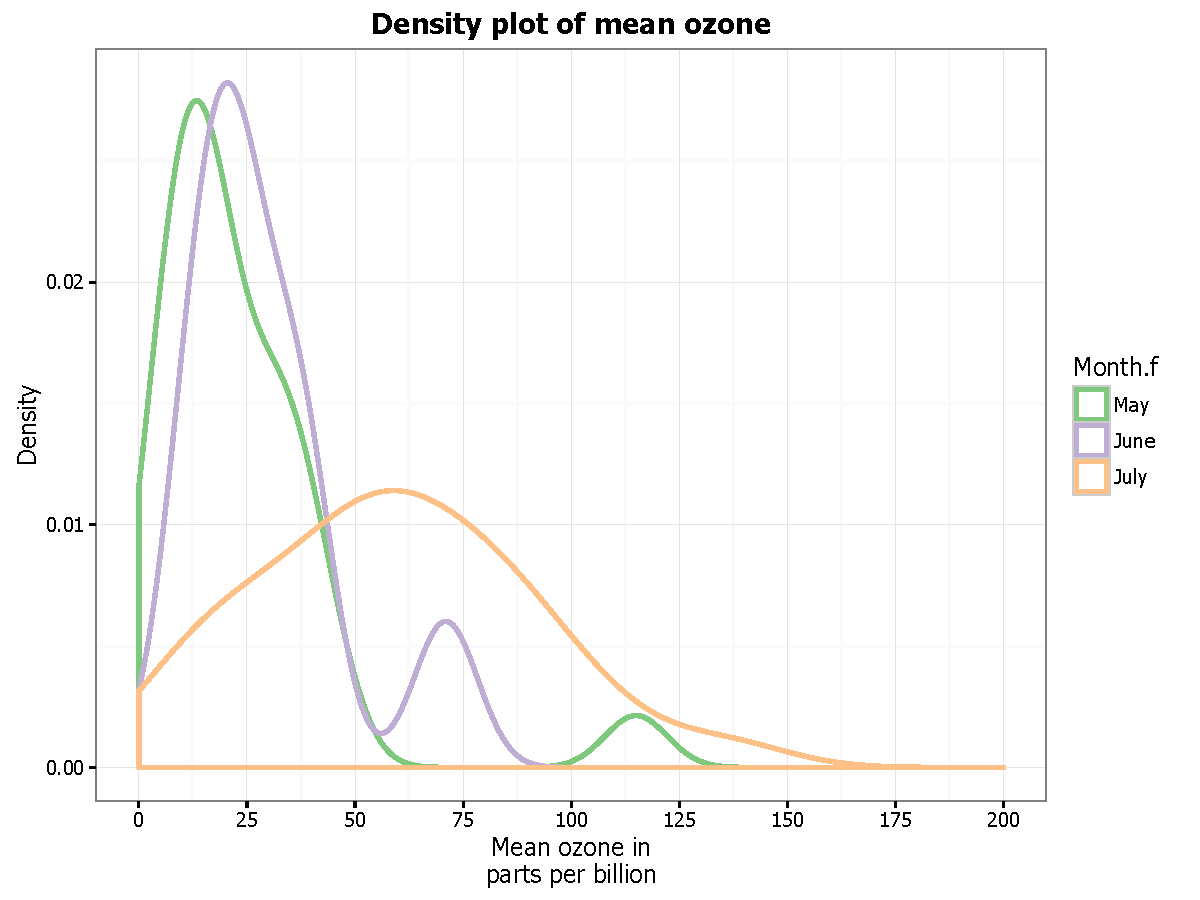
\includegraphics[width=0.55\linewidth]{figures/density_18-1} \end{center}

\section{Formatting the legend}\label{formatting-the-legend-1}

Finally, we can format the legend. Firstly, we can change the position
by adding the \texttt{legend.position\ =\ "bottom"} argument to the
\texttt{theme} option, which moves the legend under the plot. Secondly,
we can fix the title by adding the \texttt{labs(fill="Month")} option to
the plot.

\begin{Shaded}
\begin{Highlighting}[]
\NormalTok{p8 <-}\StringTok{ }\KeywordTok{ggplot}\NormalTok{(airquality_trimmed, }\KeywordTok{aes}\NormalTok{(}\DataTypeTok{x =} \NormalTok{Ozone, }\DataTypeTok{colour =} \NormalTok{Month.f)) +}\StringTok{ }
\StringTok{      }\KeywordTok{geom_density}\NormalTok{(}\DataTypeTok{position=}\StringTok{"identity"}\NormalTok{, }\DataTypeTok{fill =} \OtherTok{NA}\NormalTok{, }\DataTypeTok{size =} \DecValTok{1}\NormalTok{) +}
\StringTok{      }\KeywordTok{scale_x_continuous}\NormalTok{(}\DataTypeTok{name =} \StringTok{"Mean ozone in}\CharTok{\textbackslash{}n}\StringTok{parts per billion"}\NormalTok{,}
\StringTok{        }\DataTypeTok{breaks =} \KeywordTok{seq}\NormalTok{(}\DecValTok{0}\NormalTok{, }\DecValTok{200}\NormalTok{, }\DecValTok{25}\NormalTok{),}
\StringTok{        }\DataTypeTok{limits=}\KeywordTok{c}\NormalTok{(}\DecValTok{0}\NormalTok{, }\DecValTok{200}\NormalTok{)) +}
\StringTok{      }\KeywordTok{scale_y_continuous}\NormalTok{(}\DataTypeTok{name =} \StringTok{"Density"}\NormalTok{) +}
\StringTok{      }\KeywordTok{ggtitle}\NormalTok{(}\StringTok{"Density plot of mean ozone"}\NormalTok{) +}
\StringTok{      }\KeywordTok{scale_colour_brewer}\NormalTok{(}\DataTypeTok{palette=}\StringTok{"Accent"}\NormalTok{) +}
\StringTok{      }\KeywordTok{labs}\NormalTok{(}\DataTypeTok{colour =} \StringTok{"Month"}\NormalTok{) +}
\StringTok{      }\KeywordTok{theme_bw}\NormalTok{() +}
\StringTok{      }\KeywordTok{theme}\NormalTok{(}\DataTypeTok{legend.position =} \StringTok{"bottom"}\NormalTok{,}
\StringTok{        }\DataTypeTok{plot.title =} \KeywordTok{element_text}\NormalTok{(}\DataTypeTok{size =} \DecValTok{14}\NormalTok{, }\DataTypeTok{family =} \StringTok{"Tahoma"}\NormalTok{, }\DataTypeTok{face =} \StringTok{"bold"}\NormalTok{), }
\StringTok{        }\DataTypeTok{text =} \KeywordTok{element_text}\NormalTok{(}\DataTypeTok{size =} \DecValTok{12}\NormalTok{, }\DataTypeTok{family =} \StringTok{"Tahoma"}\NormalTok{))}
\NormalTok{p8}
\end{Highlighting}
\end{Shaded}

\begin{center}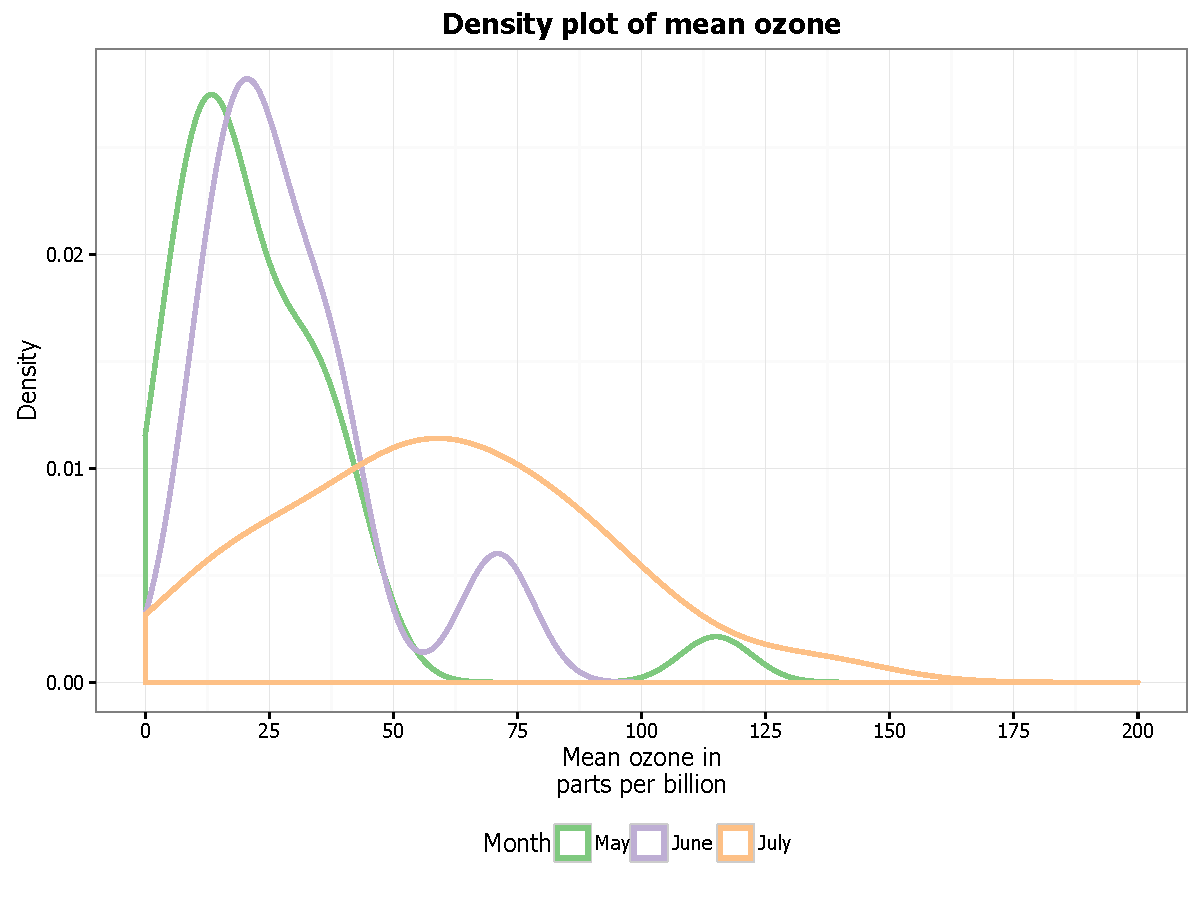
\includegraphics[width=0.55\linewidth]{figures/density_19-1} \end{center}